 % !Mode:: "TeX:UTF-8"
%!TEX program  = xelatex

\documentclass{whutmod}
\usepackage{metalogo}
\usepackage{setspace}
\usepackage{subfigure}
\usepackage{caption}
\hypersetup{
colorlinks=true,
linkcolor=black,
citecolor=black
}
\usepackage{amstext} 
\usepackage{amssymb}
\usepackage{float}
\usepackage{booktabs}
\usepackage{graphicx}
\usepackage{color}
\usepackage{amsmath}
\usepackage{gbt7714}
\usepackage{url}
\usepackage[linesnumbered,ruled,lined]{algorithm2e}


 \team{009}	% 组号
 \membera{陈凯鑫}
 \joba{编程}
 \memberb{牛 晨}
 \jobb{写作}
 \memberc{丁锦豪}
 \jobc{建模}

 \title{基于遗传退火算法的柔性车间调度方案}
 \tihao{B} % 题号

\begin{document}
\begin{spacing}{1.2}

        \date{}
%	 \maketitle
        
	\begin{center}\zihao{3}
		\textbf{基于遗传退火算法的柔性车间调度方案}
		\end{center}
	
	\begin{abstract}\setlength{\parskip}{0.3\baselineskip}
		本文分析机械公司车间生产安排问题建立了\textbf{可并行柔性车间调度模型},运用\textbf{遗传算法和模拟退火相结合}的混合方法求解,最后计算出可并行柔性车间调度方案的最优解。
		
		针对\textbf{问题一},本文建立了\textbf{柔性车间调度模型(FJSP)},采用遗传算法和模拟退火相结合的混合算法求解目标结果,得到最大完工时间的最小值。结果表明最大完工时间的最小值为\textbf{59132}分钟,并画出\textbf{甘特图}表示8台机器的具体使用情况。
		
		针对\textbf{问题二},基于问题一建立的\textbf{FJSP模型},考虑增加了某产品的提前交货情况,引进\textbf{三角模糊数},建立新的目标函数并增加约束条件,采用第一问中遗传退火的混合算法进行求解,在编码过程中采用单层编码,更能保证空闲机器的有效利用和完工时间较短。最终得到了\textbf{模糊甘特图},可以用来描述提前交货产品所带来的影响程度大小。
  
	    针对\textbf{问题三},基于问题一建立的FJSP模型,新增目标函数与约束条件,建立\textbf{多目标动态规划模型},采用单层编码的\textbf{遗传与模拟退火相结合的混合算法}进行求解得到具有一般适用性的生产计划方案。考虑各机床的停工时间尽量少和最终完工时间尽量短两个目标,对产品进行\textbf{分批调度},将使各个机床的停工时间最少这个目标转化为每个工件的最后一道工序在对应的机器上完成的时刻之和最小。最终得到两种\textbf{甘特图}来衡量在产品数目以及机床数目都可能增加的情况下可并行柔性车间调度方案的最优解。

       本文\textbf{优点}:(1)将遗传算法与模拟退火算法相结合取
       各自算法的优点得到混合算法来求解模型。
         (2)在交叉过程中,相比于以往固定的交叉概率和变异概率,本文采用动态自适应的交叉概率和变异概率,可以加快算法收敛。
		
		
		
		 %本文\textbf{优点}:(1)利用lightGBM特征重要性选择法,巧妙的证明了主要变量的合理性.
		 %(2)综合比较多种预测算法,使得预测误差更小.
		 %(3)充分考虑实际情况建立熵权topsis模型进行风险评估.
		
		
		
		

		\keywords{
		    柔性车间调度模型(FJSP)\quad 遗传退火混合算法\quad 甘特图\quad 三角模糊数\quad 多目标动态规划模型\quad
		  
			
			
		}
		
	\end{abstract}

    \thispagestyle{empty}
	\tableofcontents
	\thispagestyle{empty}

	\newpage
	\setcounter{page}{1}

	\section{问题重述}
    


	\subsection{问题背景}

    近年来,随着我国科学技术的不断发展,传统的制造业正在向着自动化、数字化的方向迈进,引领了智能制造发展的新趋势。车间调度问题则是生产制造的一个重要环节,车间作业调度是对车间生产过程进行作业计划,使生产制造业实现智能化、自动化、信息化的核心,而且是车间作业系统生产管理的核心部分,因此如何有效地分配生产工序,使用合理的科学方案,来优化生产目标,减少加工时间和加工成本已经成为了制造企业重点关注的热点问题。本文是通过分析某机械公司成产车间的实际情况与具体要求,建立数学模型对其成产过程进行优化,并给出了具有一般适用性的生产计划方案。
    	\begin{figure}[H]
        \centering
        
\includegraphics[width=0.7\textwidth]{智能车间生产图.png}
        \caption{智能车间生产图}
    \end{figure}


	\subsection{问题提出}
   该车间实际成产情况为为9件产品需要在8台机器上进行加工,每个产品包含2-4道工序,工序之间包含或并行或前后制约的关系,并且可以在不同的机器上进行加工,基于以上限制来解决下列问题:
    
\textbf{问题1:}建立优化模型,并构造求解该优化模型的算法,目标为使得整个车间系统加工完目标产品数量的时间最小。

\textbf{问题2:}在第一问的算法中进行修改,考虑如有产品需要提前交货,既要保证提前交货的产品能按时完工,还需考虑总加工时间较短,应如何合理安排生产计划。

\textbf{问题3:}在第一问算法中改进,尽量减少各机床的空闲时间,进而实现高的设备利用率。并在产品数目以及机床数目都可能增加的情况下,建立合理的数学模型,构造求解算法给出具有一般适用性的生产计划方案。



	\section{模型的假设}

	\begin{itemize}
	\item 假设每种产品分一个批次进行加工,该批次数量为本月需求量。
		
		
    \item 假设每台机床一次只能加工一个产品的某一道工序。

     \item 假设某一类产品的某一道加工工序在某几台机床上进行时,这些机床是没有差的,单品加工时间以及切换时间全部相同。

      \item 假设每道工序之间可能存在先后顺序关系,即该产品在完成某一道工序后才能F始下一道工序;也可能存在并列关系,即该产品在某一道工序完成后可以选择t进行后两道不同的工序中的任意一道。

    
    
    
	\end{itemize}

    \section{符号说明}
    \begin{center}
    \begin{tabular}{cc}
     \toprule[1.5pt]
     \makebox[0.3\textwidth][c]{符号}	&  \makebox[0.4\textwidth][c]{含义} \\
     \midrule[1pt]

     $M_{j}$         & 第j道工序的可使用机器集合\\
     $P_{ijk}$        & 工件i的工序j在机器k上加工所需时间\\
     $S_{ijk}$          &  工件i的工序j在机器k上的开始加工时\\
     $C_{ijk}$        & 工件i的工序j在机器k上的结束加工时间\\
     $N_{jk}$         &工序j在机器k上加工的工件数量\\
     $R_{jk}$         &在工序j的机器k上进行加工的第R个工件\\
     $x_{ijk}$         &检验工件i的工序j在机器k上进行加工的指\\
     $f$         &特征变量\\
     $J_i$        &第i个产品\\
     $O_{ij}$        &第$i$个产品的第j个工序\\
     $D_i$   &第$i$个机器\\
     $f_a$   &平均适应度\\
     $H_{ij}$     &第 i 个工件的第 j 道工序的切换时间\\
     $M$  &分批次数\\
      
      
     
     
     
    \bottomrule[1.5pt]
    \end{tabular}
    \end{center}

	\clearpage

    
    
	
	\section{问题一模型的建立与求解}

	\subsection{问题一的分析}
	该问题为典型的车间调度问题(JSP)\cite{2},并且由于该车间的某一产品可以在任何一个可用机器上进行处理,所以为柔性车间调度问题(FJSP),并且还存在着可以并行加工的工序,需要对传统的FJSP问题的解决方法进行改进。我们需要解决两个问题:确定各作业的加工先后顺序和机器选择。本文利用遗传算法与模拟退火相结合的混合算法,调度优化产品与工序在机器上加工的顺序,使整个系统的加工时间最小。问题一分析流程图如下:
	\begin{figure}[H]
        \centering
        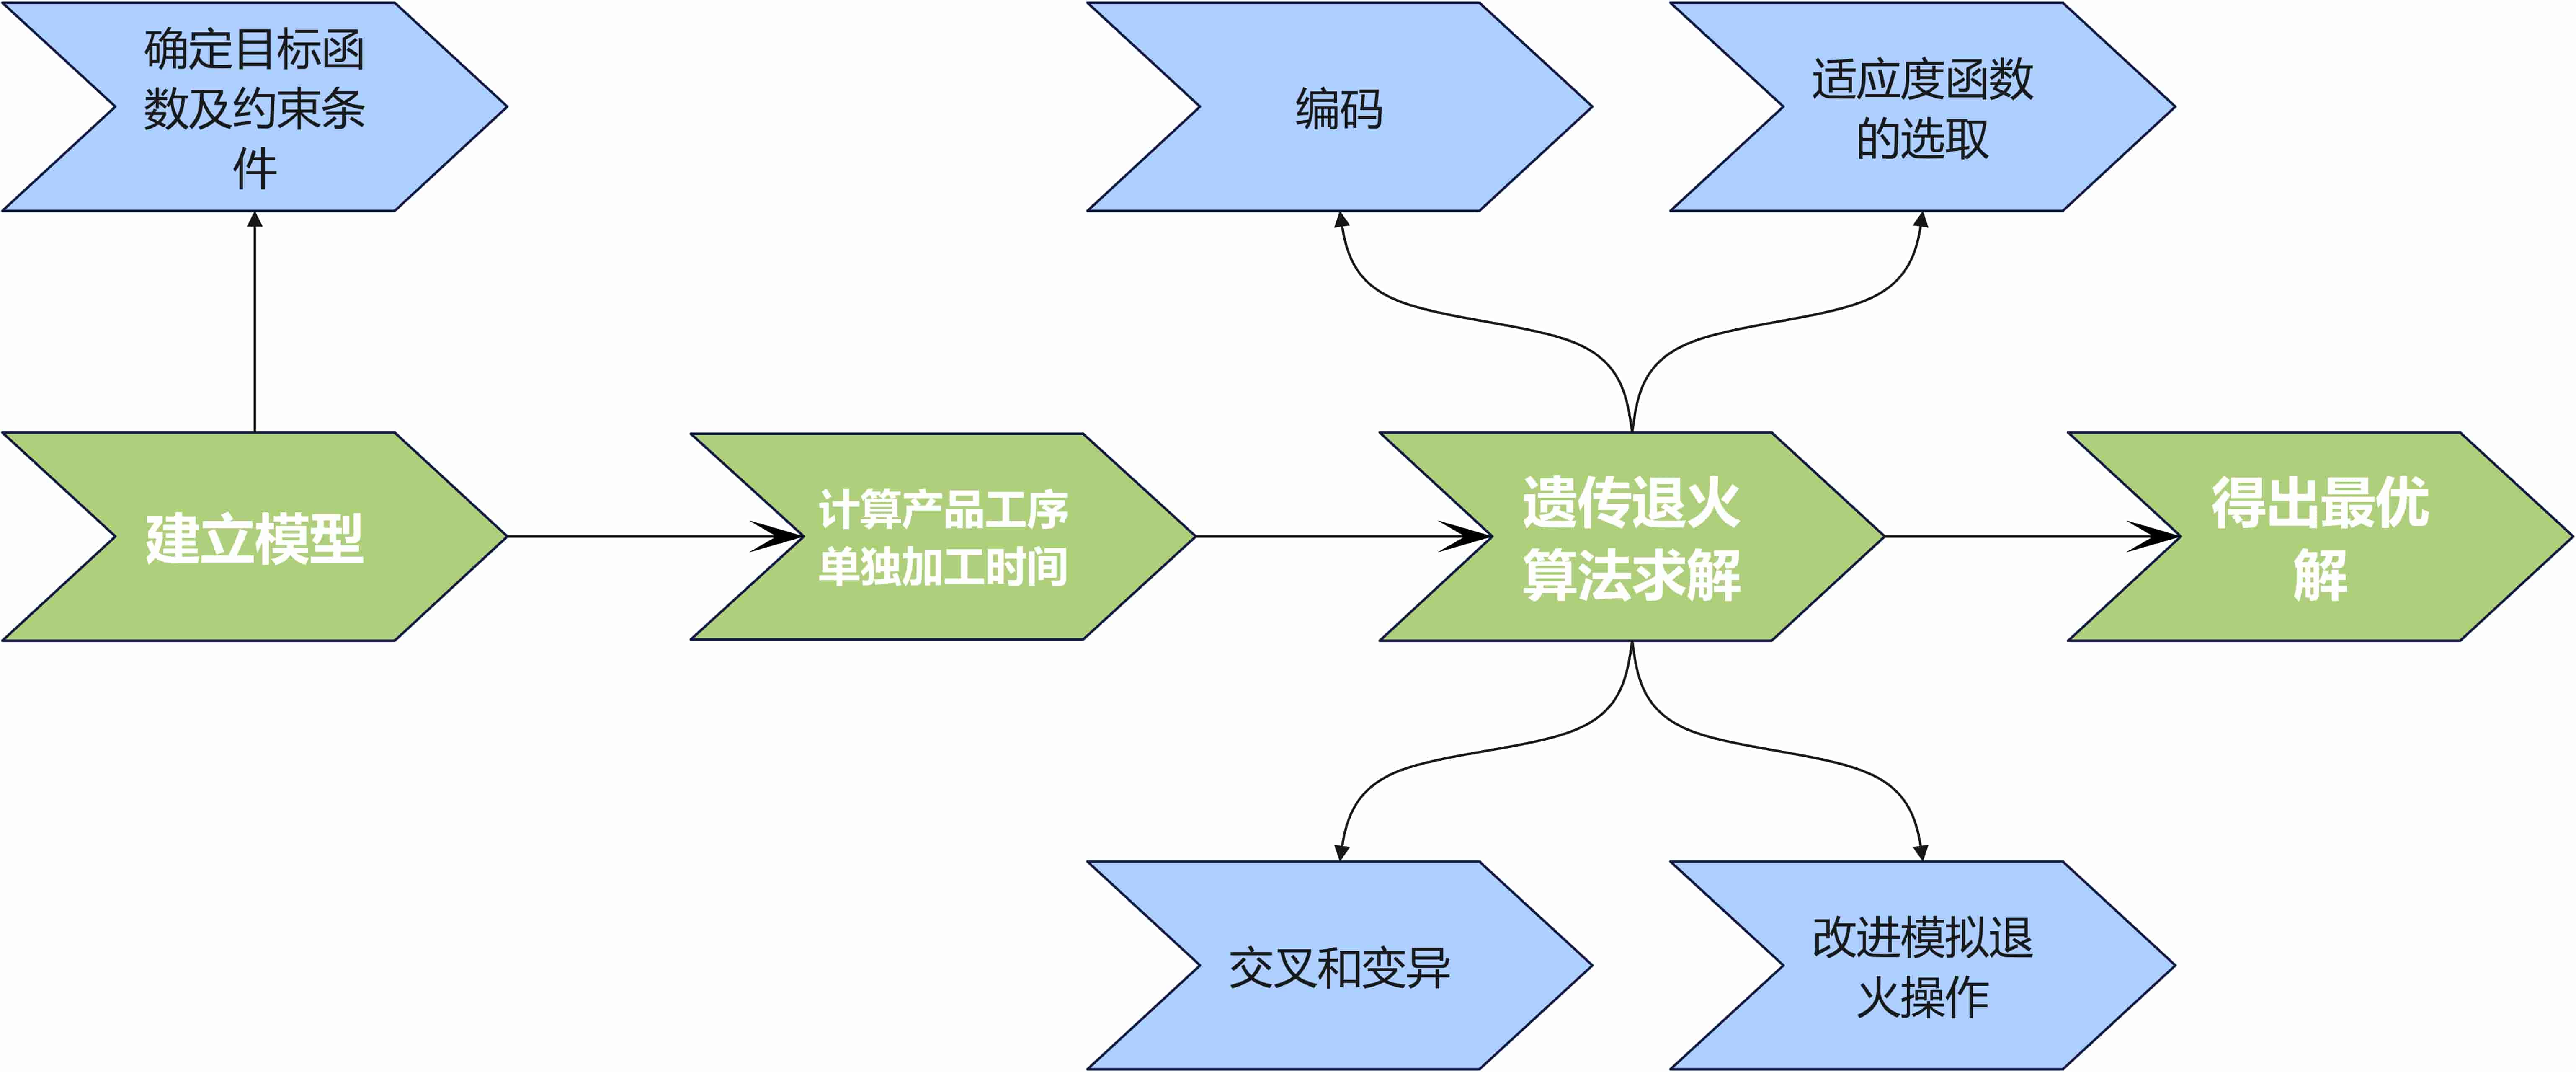
\includegraphics[width=0.9\textwidth]{模型一流程图.jpg}
        \caption{问题一的分析}
    \end{figure}

其中,不同工序可选机器如下表所示:
 
	\begin{center}
   	\begin{table}[H]
   		\centering
   		\caption{不同工序可选机器表}
   		\begin{tabular}{cccccccccc}
   			\toprule[1.5pt]
   			\makebox[0.07\textwidth][c]{}	&   
            \makebox[0.07\textwidth][c]{产品1}	&
   			\makebox[0.07\textwidth][c]{产品2}	&
            \makebox[0.07\textwidth][c]{产品3}	&
            \makebox[0.07\textwidth][c]{...}	&
            \makebox[0.07\textwidth][c]{产品7}	&
            \makebox[0.07\textwidth][c]{产品8}	&
   			\makebox[0.07\textwidth][c]{产品9}		\\
   			\midrule[1pt]
   			工序1  & [BCD] &  [FG]   &[FGHE] & ...&  [ABCD]& [EFGH]&  [ABCD]   \\
   		    工序2  & [BCD] &  [FG]   & [BCD] &...&  [ABCD]& [EFGH]&  [ABCD]\\
   			工序3  & [FG] &  [BCD]  & [FGHE]  &...&  [BCD]& [BCD]&  - \\
   			工序4  & [BCD] &  -  & -      & ...& [ABCD]& [ABCD]&  -\\
   			\bottomrule[1.5pt]
   		\end{tabular}
   	\end{table}
   \end{center}

不同机器完成各项产品不同工序所需时间如下表所示:
       

	    
	   \begin{center}
   	\begin{table}[H]
   		\centering
   		\caption{机器加工不同工序所需时间表}
   		\begin{tabular}{cccccccccc}
   			\toprule[1.5pt]
   			\makebox[0.04\textwidth][c]{}	&   
            \makebox[0.04\textwidth][c]{产品1}	&
   			\makebox[0.04\textwidth][c]{产品2}	&
            \makebox[0.04\textwidth][c]{产品3}	&
            \makebox[0.05\textwidth][c]{...}	&
            \makebox[0.05\textwidth][c]{产品7}	&
            \makebox[0.05\textwidth][c]{产品8}	&
   			\makebox[0.05\textwidth][c]{产品9}		\\
   			\midrule[1pt]
   			工序1  & [11553] &  [17380]   &[8410] & ...&  [9405]& [4975]&  [11430]   \\
   		    工序2  & [5769] &  [19770]   & [15885] &...&  [11665]& [4975]&  [9155]\\
   			工序3  & [4657] &  [4905]  & [3902]  &...&  [18910]& [7395]&  - \\
   			工序4  & [2616] &  -  & -      & ...&  [5375]& [2857]&  -\\
   			\bottomrule[1.5pt]
   		\end{tabular}
   	\end{table}
   \end{center}
	

	\subsection{FJSP模型的建立和求解}
	\subsubsection{FJSP模型的建立}
	标准柔性车间调度问题可以描述为:有n个工件在m台机器上加工,每个工件有一道或者多道加工工序,每道工序可以有多种可选择的加工机器,但不同的机器加工工件所需时间不同\cite{3}。调度方案需要在满足加工先后顺序约束的情况下,选择合适的机器对工件进行加工,优化各机器上加工顺序,使得最大完工时间最小。但该车间允许部分的工序并行使用,就需要限制约束条件,使可以并行的工序尽量并行进行来节省时间。
    以最小化最大完工时间为优化目标建立数学模型,其目标函数为:

\begin{gather}
		min\left ( max\left ( C_{ijk}  \right )  \right ) 
	\end{gather}
 其中$C_{ijk}$表示工件 i 的工序 j 在机器 k 上的结束加工时间。

此外,还需要满足以下约束条件:
\begin{gather}
\sum_{k=1}^{M_{j}}x_{ijk} =1
 \end{gather}

其中$M_{j}$表示第 j 道工序的可使用机器集合,$x_{ijk}$表示检验工件 i 的工序 j 在机器 k 上进行加工的指标,如下式:

\begin{gather}
x_{ijk} =\left\{\begin{matrix}   1, \mbox{工件i的工序j在机器k上进行加工}\\   0,\mbox{其他}  \hfil\end{matrix}\right. 
\end{gather}
此式表示同一时间内每道工序只能被一台机器加工;


\begin{gather}
\sum_{k=1}^{M_{j}}N_{jk} =n
\end{gather}

其中,$N_{jk}$为工序 j 在机器 k 上加工的工件数量,n为工件数量,表示对每道工序,分配给工序内所有机器的工件数之和为n;

\begin{gather}
C_{ijk} \le S_{i\left ( j+1 \right )r} ,r\in M_{j+1} ,f\in ( 0,1)
\end{gather}

其中,$C_{ijk}$为工件 i 的工序 j 在机器 k 上的结束加工时间,该式表示同一工件在进行加工时必须遵循加工先后约束,即只有完成上一道工序的加工后,才能开始下一道工序的加工,由于该问题允许部分工序同时并行加工,我们选取f为特征变量,用来表示该式是否需要成立,当出现产品1的2工序和3工序、产品4的2工序和3工序、产品5的2工序和3工序、产品6的3工序和4工序、产品7的3工序和4工序、产品8的3工序和4工序这六种情况时,特征变量f为0,表示上式的约束条件可以忽略;其余情况特征变量f为1,上式的约束条件必须遵守。

\begin{gather}
C_{ijk} = S_{ijk} +  P_{ijk} 
\end{gather}

其中$P_{ijk}$工件 i 的工序 j 在机器 k 上加工所需时间,该式表示工件的结束加工时间为工件开始加工时间与该工序加工所需的时间之和。

\begin{gather}
C_{r_{jk} jk} \le  S_{\left ( R+1 \right )_{jk}  jk} , R=1,2,3,...,N_{jk} -1
\end{gather}

该式表示表示同一时间每个机器只能加工一个工序。

\begin{gather}
x_{ijk} \in \left \{ 0,1 \right \} ;\forall i,j,k  
\end{gather}

\begin{gather}
f \in \left \{ 0,1 \right \}  
\end{gather}

该式表示变量取值范围。

综上为针对问题一建立的FJSP优化模型:

目标函数为:

\begin{gather}
		min\left ( max\left ( C_{ijk}  \right )  \right ) 
	\end{gather}

 约束条件为:

 \begin{gather}
		\left\{\begin{matrix}   \sum_{k=1}^{M_{j}}x_{ijk} =1 \\    \sum_{k=1}^{M_{j}}N_{jk} =n \\C_{ijk} \le S_{i\left ( j+1 \right )r} ,r\in M_{j+1} ,f\in ( 0,1)\\C_{ijk} = S_{ijk} +  P_{ijk} \\ C_{r_{jk} jk} \le  S_{\left ( R+1 \right )_{jk}  jk} , R=1,2,3,...,N_{jk} -1 \\x_{ijk} \in \left \{ 0,1 \right \} ;\forall i,j,k  \\f \in \left \{ 0,1 \right \}  \end{matrix}\right. 
	\end{gather}
    
	\subsubsection{基于遗传与模拟退火相结合的算法求解模型}

遗传算法是一种解决大规模计算问题的全局搜索方法\cite{4},通过模拟自然进化过程搜素最优解。遗传算法虽然全局搜索能力极强,但其局部搜索能力差,而模拟退火算法是一种贪心算法,通过模拟物理降温过程,它的搜索过程引入了随机因素,以一定的概率来接受一个比当前解要差的解,因此有可能会跳出这个局部的最优解,达到全局的最优解,其结果受其最优解会受到迭代次数k的影响,但该算法存在收敛速度慢,耗时较长的问题。为了充分利用两种算法各自的优点,本文采用遗传与模拟退火相结合的混合算法来进行求解,即先使用遗传算法求出初始解,然后使用模拟退火算法\cite{1}搜索更优的解,进一步得到车间最大完工时间的最小值。改进遗传模拟退火算法具体步骤如下:

STEP1:初始化参数,生成初始种群。

STEP2:对种群进行染色体编码。 

STEP3:确定自适应函数 进行交叉和变异操作,随机选择染色体个别位置 相互交换,在此基础上采用动态自适应的交叉率和变异率, 加快算法收敛。

STEP4:进行交叉和变异操作,随机选择染色体个别位置 相互交换,在此基础上采用动态自适应的交叉率和变异率, 加快算法收敛。 

STEP5:将交叉变异后的种群进行模拟退火操作,避免陷入局部最优解。

STEP6:将模拟退火后的优异个体重新进行适应度值计算。

STEP7:判断是否达到迭代条件,若达到迭代条件,结束并输出最优解;否则,转至步骤5。

\begin{itemize}
	    \item[\textbf{1.}] \textbf{算法编码}
	\end{itemize}

 在对FJSP进行编码过程中采用工件排序和机器选择两个步骤,第一步是对工件的加工顺序进行合理的排列,第二步是根据工件的加工顺序,选择合适的机器进行加工,使得工件的加工时间最小。采用了双层整数编码来表示这个过程,第一层编码是工件加工顺序 (OperationSequence, OS),第二层编码是机器分配序列(Machine Assignment, MA)。具体编码方式如下图所示:
 
		\begin{figure}[H]
		\centering
		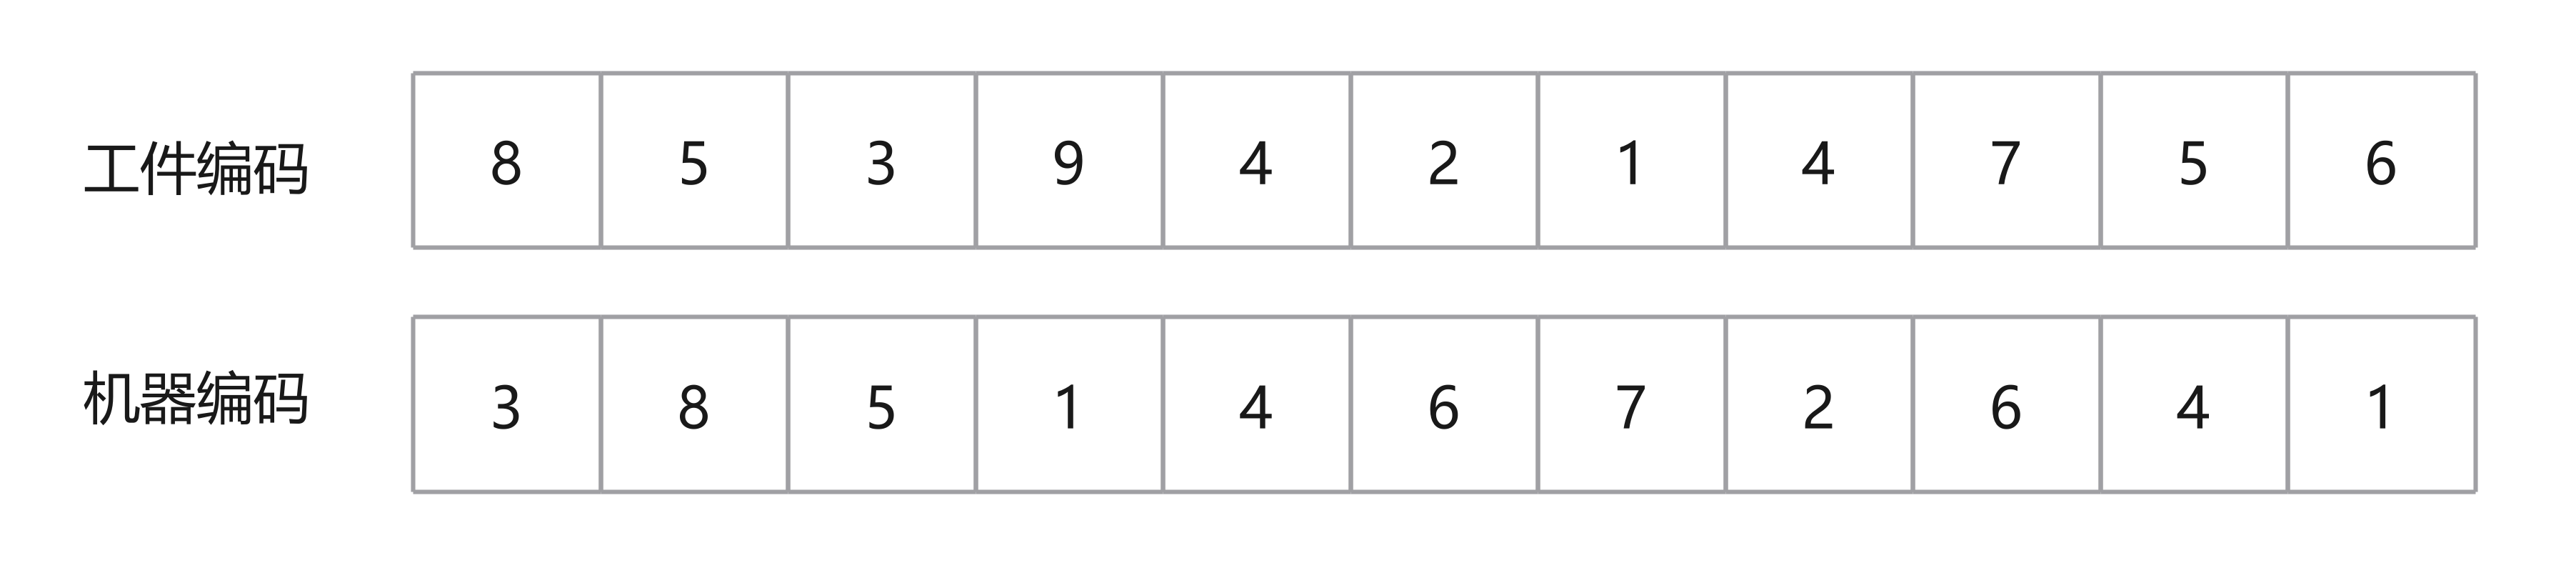
\includegraphics[width=0.8\textwidth]{编码.png}
		\caption{双重编码图}
	\end{figure}

上图说明了在第一层的工件编码中,第一次出现的数字为产品的第一道工序,第二次出现的数字为该产品的第二道工序,以此类推。第二层工件编码的数字则说明了在第一层中编码的某个产品的某道工序是在哪个机器上加工的,其中数字1-8代表了机器A-H,例如,第一行的第8个数字4,因为它是第二次出现的,所以代表了其为产品4的第二道工序,其对应的机器编码是2,说明是在B机器上加工了4产品的第二道工序。这样通过编码的方式,可以将模型与算法联系起来并进行求解。

\begin{itemize}
	    \item[\textbf{2.}] \textbf{适应度函数的选取}
	\end{itemize}

 由于问题一中要求我们得到最大完工时间的最小值,所以我们的适应性函数可以直接选取目标函数。
 即:

 \begin{gather}
		min\left ( max\left ( C_{ijk}  \right )  \right ) 
	\end{gather}

 \begin{itemize}
	    \item[\textbf{3.}] \textbf{交叉和变异}
	\end{itemize}
 
 \begin{itemize}
	    \item 交叉规则
     
为避免产生非法解,本次研究采用工序和设备单独交叉形式,首先对工序进行单独交叉,设备跟随工序;然后,随 机选择设备进行单独交叉。交叉的具体步骤如下。 

  STEP1:工序交叉,设备跟随,如下图所示:

  \begin{figure}[H]
		\centering
		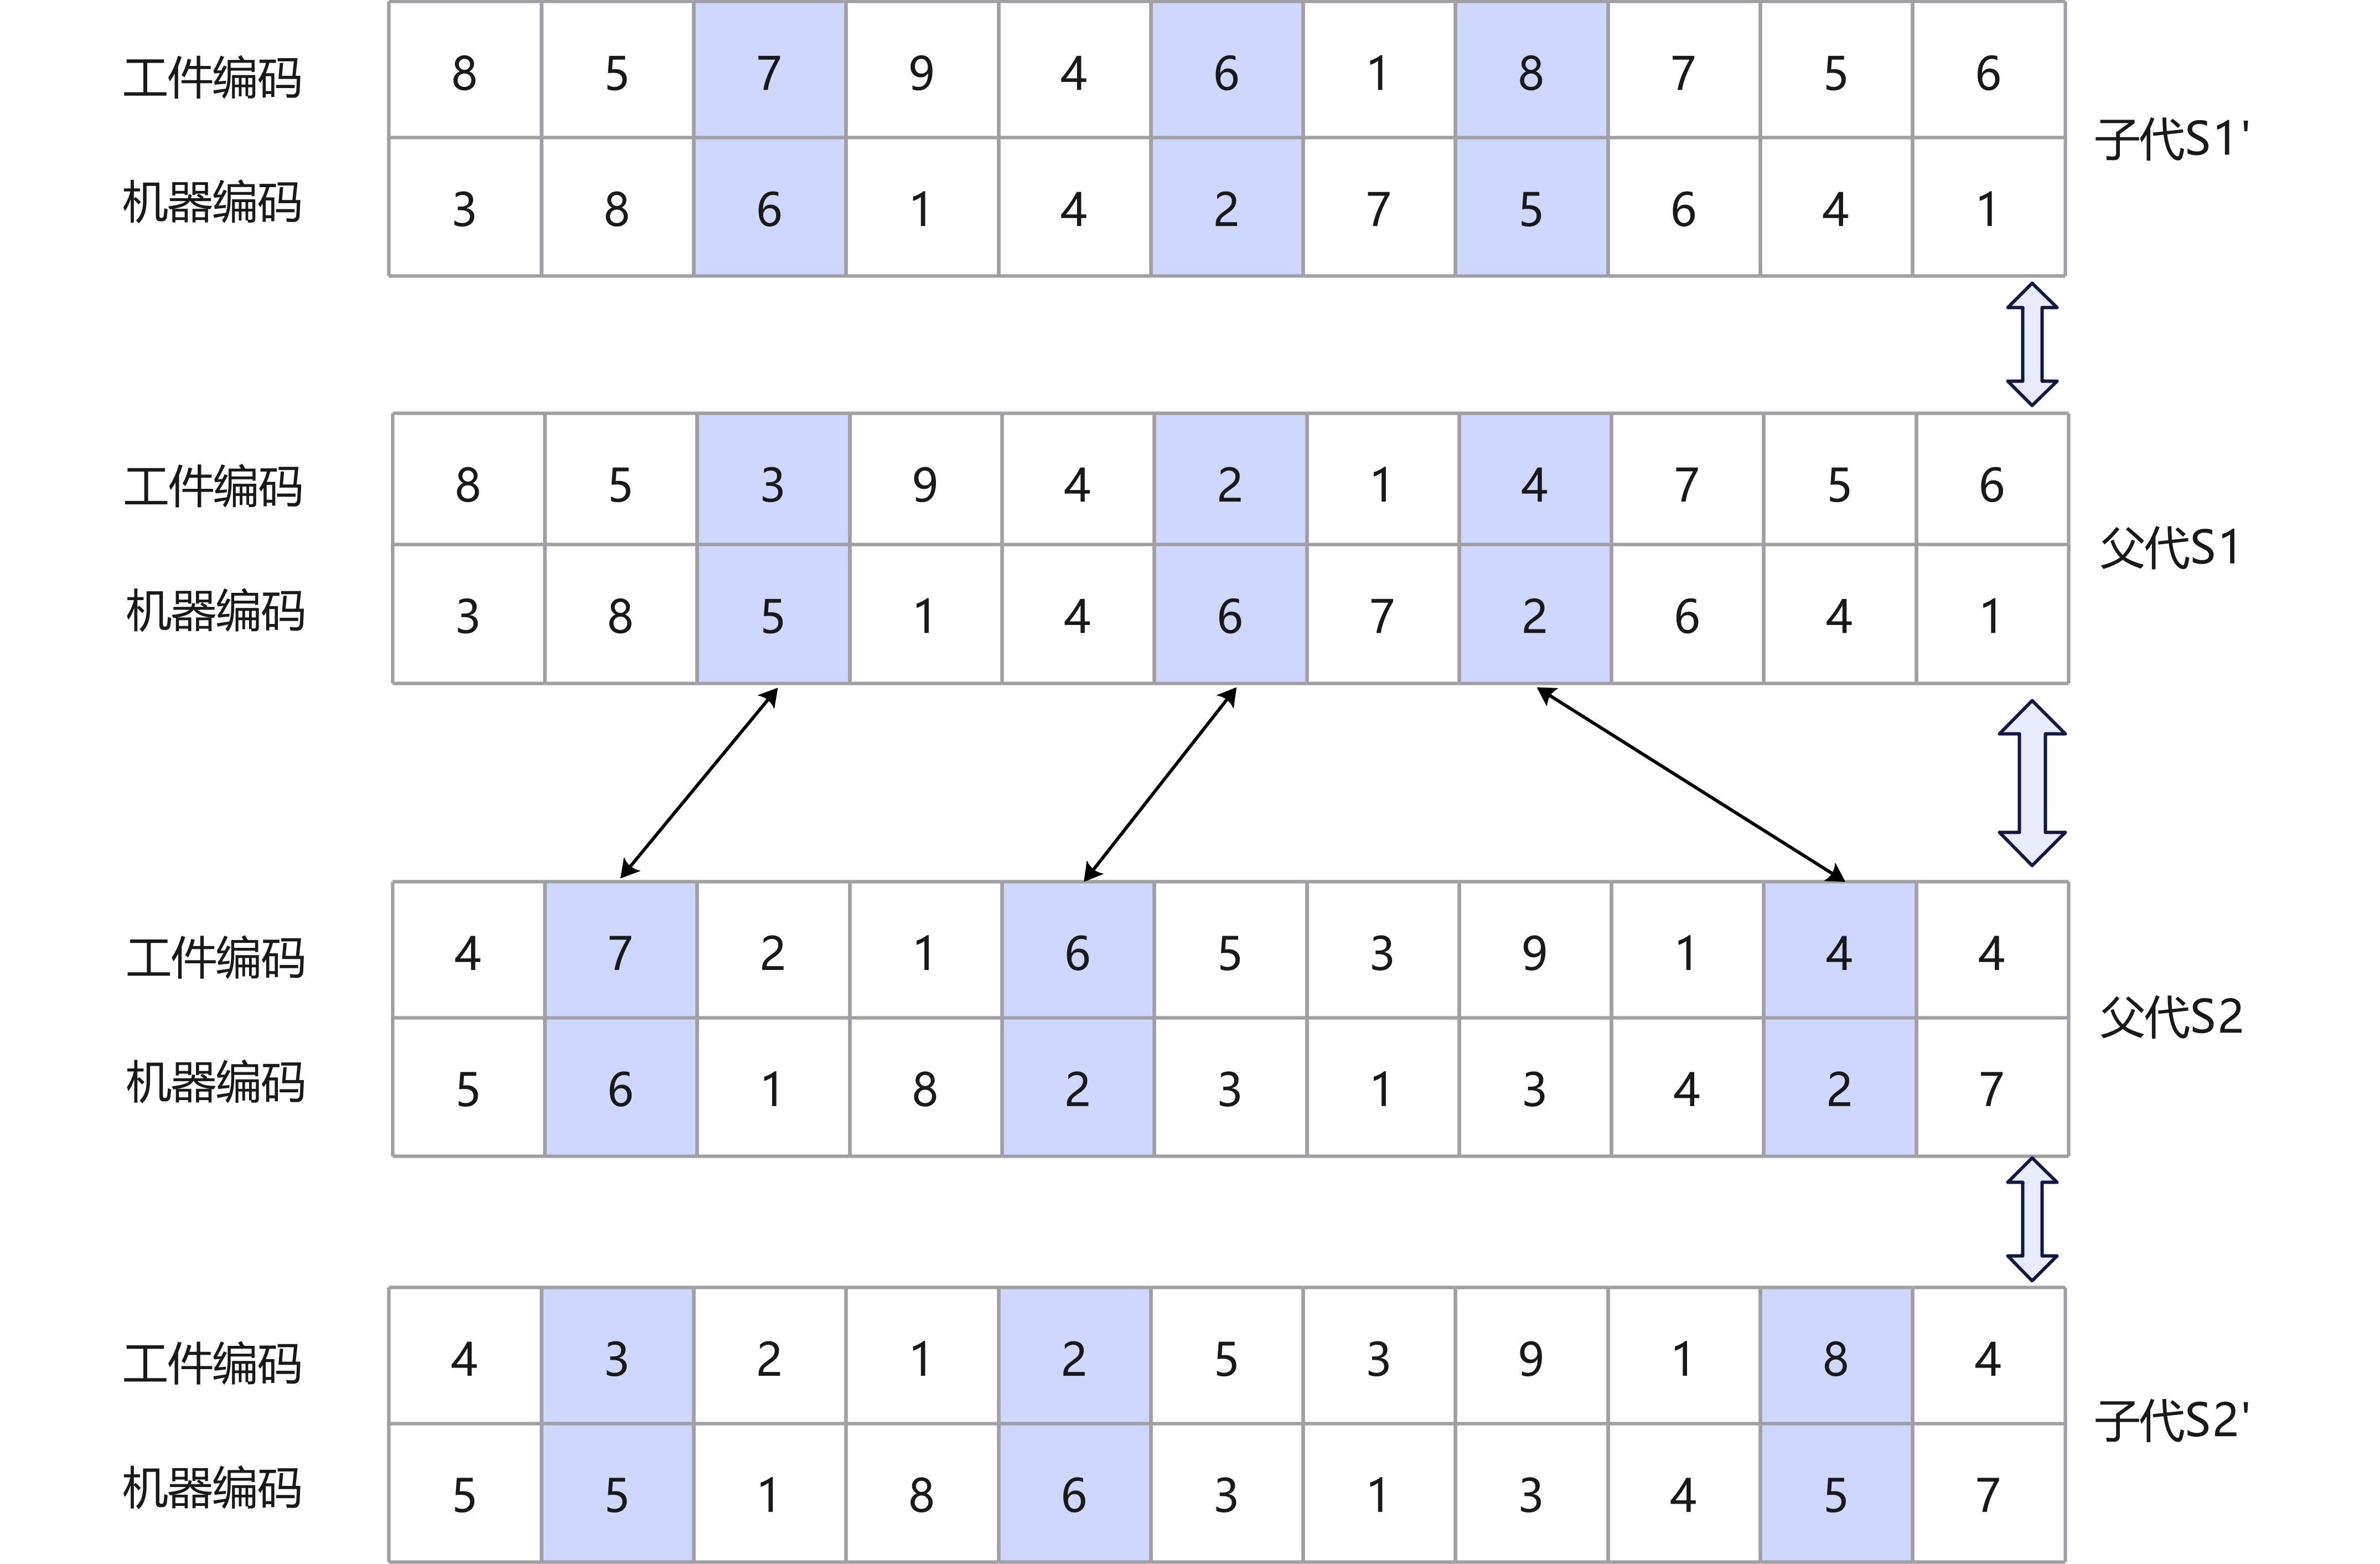
\includegraphics[width=0.8\textwidth]{工序交叉.jpg}
		\caption{工序交叉图}
	\end{figure}


  STEP2:设备单独交叉,如下图所示:

  \begin{figure}[H]
		\centering
		\includegraphics[width=0.8\textwidth]{机器交叉.jpg}
		\caption{机器交叉图}
	\end{figure}


        \item 变异规则

        在两个个体中随机选择两个位置进行交换。若交换的两个位置是相同工序码,则需要从父代中将与该工序编号相同的列依次取出,并按顺序依次插入到子代相应位置,如下图所示:


        \begin{figure}[H]
		\centering
		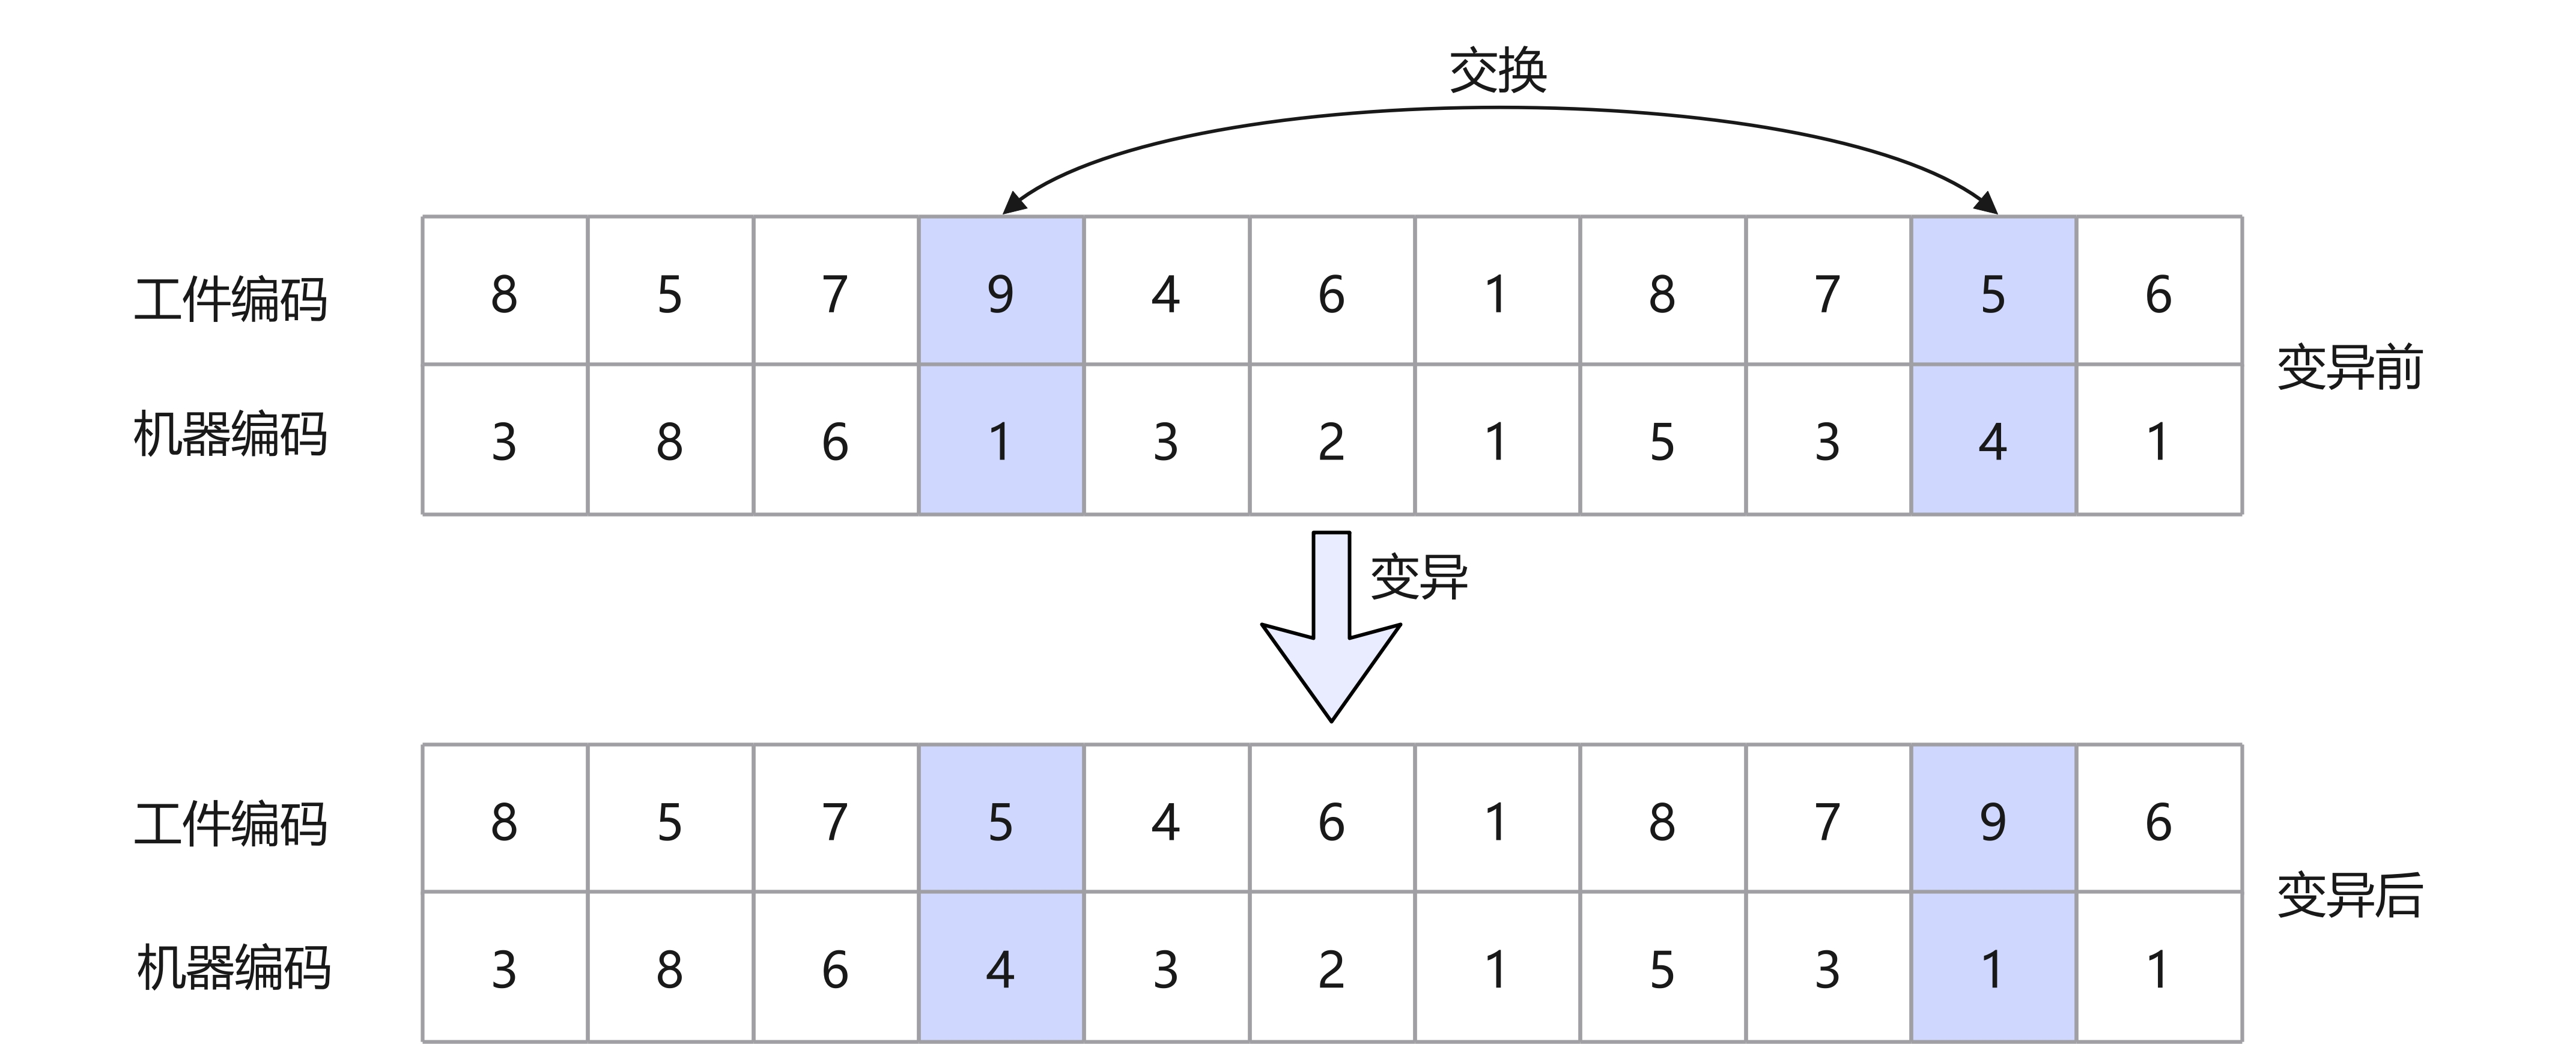
\includegraphics[width=0.8\textwidth]{变异.jpg}
		\caption{变异过程图}
	\end{figure}
  
        \item 改进自适应交叉率和变异率

        在以往的交叉环节中,往往采用确定的交叉概率和变异概率,容易导致早熟收敛等问题。为提高自适应能力,提出动态自适应交叉率和变异率,通过适应度值大小来进行调整,加快算法收敛,公式如下:

\begin{gather}
		u= \frac{\pi }{2\left ( N-1 \right )^{v}  } \left ( i-1 \right ) ^{}
	\end{gather}

\begin{gather}
		P_t=\left\{\begin{array}{cc}
\cos (u) \frac{k_c\left(f_c-f_a\right)}{f_{\max }-f_a} & f_c>f_a \\
k_c & f_c \leqslant f_a
\end{array}\right.
	\end{gather}

\begin{gather}
		P_m=\left\{\begin{array}{cc}
\cos (u) \frac{k_m\left(f_m-f_a\right)}{f_{\max }-f_a} & f_m>f_a \\
k_m & f_m \leqslant f_a
\end{array}\right.
	\end{gather}

     
	\end{itemize}



其中,$k_c$和$k_m$为常数;$f_c$和$f_m$分别为两个交叉和变异个体较大的适应度值;v为调整参数;$f_a$为平均适应度值;$f_max$为种群最大的适应度值。i为已经迭代的次数,N为总的迭代次数;$P_t$和$P_m$分别为交叉概率和变异概率。

 \begin{itemize}
	    \item[\textbf{4.}] \textbf{交叉和变异}
	\end{itemize}

 使用遗传算法在交叉和变异后容易陷入局部最优解\cite{8}, 因此加入改进模拟退火算法来提高解的搜索效率,利用 Metropolis准则来判断是否接受新解,保留优良的基因片段,保证解的质量和多样性。以往的局部搜索比较耗时,改进模拟退火算法是在原算法基础上加入了基于逆序的局部搜索方法,即在得到最新当前解并降温后随机选择编码的两个不同位置并进行顺序逆转,将得到的新个体进行增量计算,判断是否将新解保留或替换,并继续循环,达到终止条件后结束,流程图如下:

  \begin{figure}[H]
		\centering
		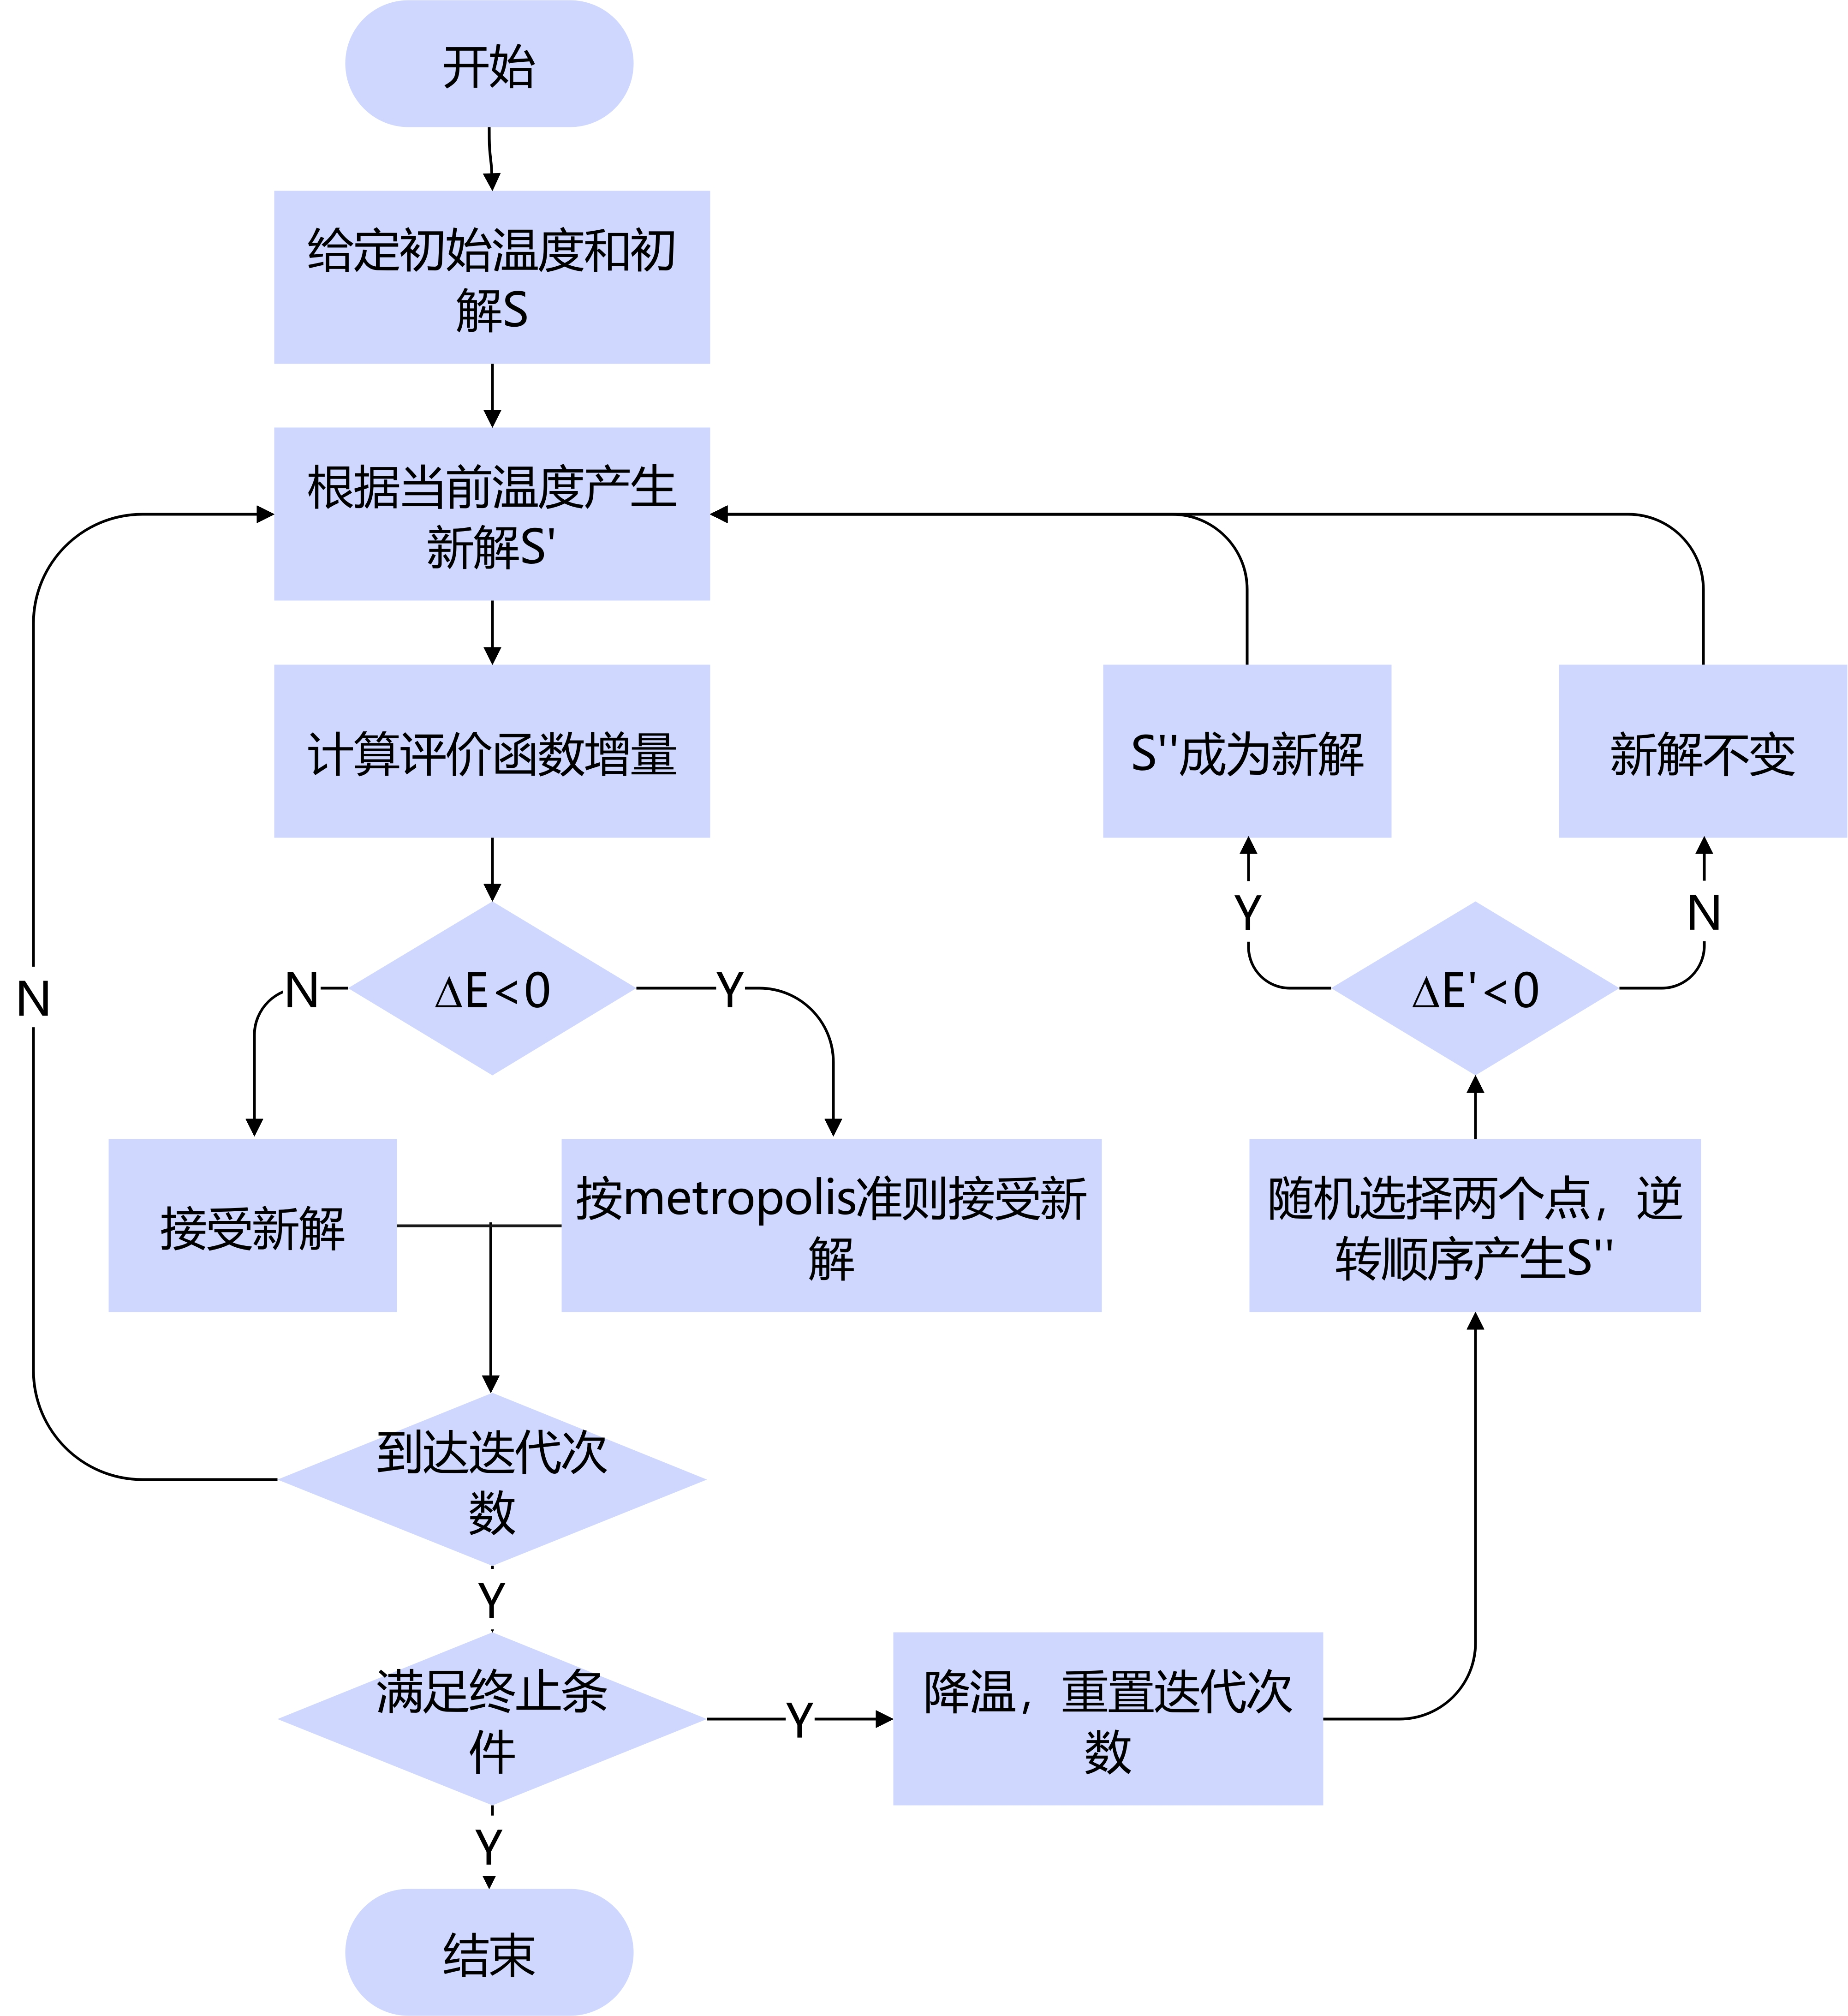
\includegraphics[width=0.6\textwidth]{问题一算法.jpg}
		\caption{遗传模拟退火流程图}
	\end{figure}
 





	
	
	
	
	

    \subsection{结果分析}
    \subsubsection{算法比较}
    为了检验采用的算法在计算结果方面是否准确,采用了差分进化算法(Differential Evolution Algorithm,DE)、遗传算法(Genetic Algorithm,GA)、粒子群(Particle Swarm Optimization, PSO)\cite{7}与本文采用的遗传与模拟退火结合的混合算法(GA+SA)的结果进行对比,比较结果如下表所示:
    
    \begin{center}
    	\begin{table}[H]
    		\centering
    		\caption{模型预测各误差对比}
    		\begin{tabular}{cccc}
    			\toprule[1.5pt]
    			\makebox[0.12\textwidth][c]{算法名称}	&   
                \makebox[0.12\textwidth][c]{平均值}	&
    			\makebox[0.12\textwidth][c]{最优解}	&
    			\makebox[0.12\textwidth][c]{最差解}		\\
    			\midrule[1pt]
    			DE    &   68840  &  65023 &	72658  \\
    			GA    &  72548  &	67842 &  77254 \\
    			PSO   &	 66736   &	63648 &  69824  \\
    			GA+SA &	 63691 &  59132 & 68250\\
    			
    			\bottomrule[1.5pt]
    		\end{tabular}
    	\end{table}
    \end{center}
    
    由表中结果可知,采用的遗传与模拟退火结合的混合算法在最优解、最差解和平均值都比上述其他三种方法得到的结果优秀,可以证明算法较为正确。


    \begin{figure}[H]
		\centering
		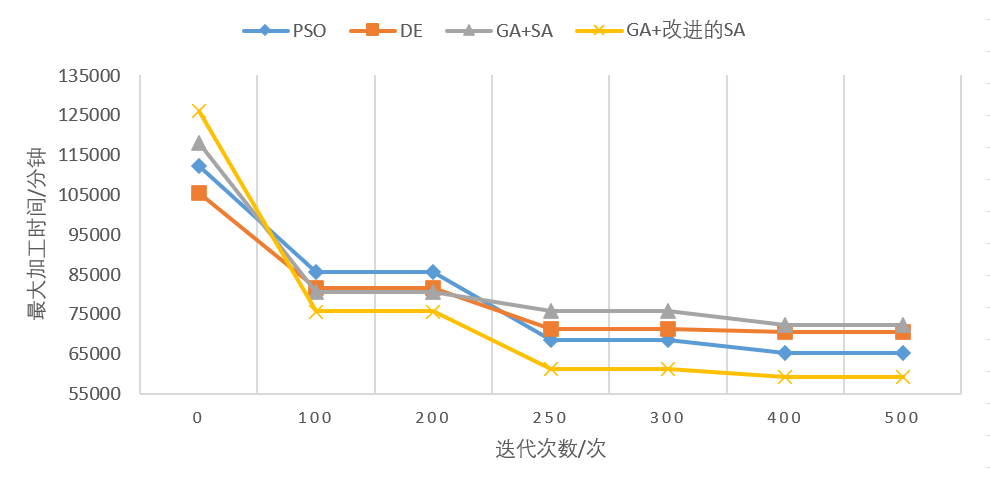
\includegraphics[width=0.8\textwidth]{算法比较图.png}
		\caption{算法比较图}
	\end{figure}
   
  由上图可知,基于GA改进的SA算法求出最大加工时间受迭代次数的变化最明显,并且最后得到的最大加工时间最小,证明了基于GA改进的SA算法求出的最优解明显优于其他三种算法。
  

\subsubsection{求解结果}

首次在遗传算法和模拟退火算法中分别调试参数,确定的具体参数如下表所示:
 
\begin{center}
    	\begin{table}[H]
    		\centering
    		\caption{算法相关参数的确定}
    		\begin{tabular}{cc}
    			\toprule[1.5pt]
    			\makebox[0.3\textwidth][c]{所需参数}	&   
                \makebox[0.12\textwidth][c]{具体值}		\\
    			\midrule[1pt]
    			种群大小    &   50   \\
    			交叉概率    &   动态改变  \\
    			变异概率   &	   动态改变   \\
    			初始温度   &	   1000 \\
                终止温度   &	   $e^{-3}$  \\
                温度衰减系数   &	 0.9 \\
    			\bottomrule[1.5pt]
    		\end{tabular}
    	\end{table}
    \end{center}



    将参数确定后直接代入程序进行求解,得到的收敛曲线如下图所示:
    
    
    \begin{figure}[H]
		\centering
		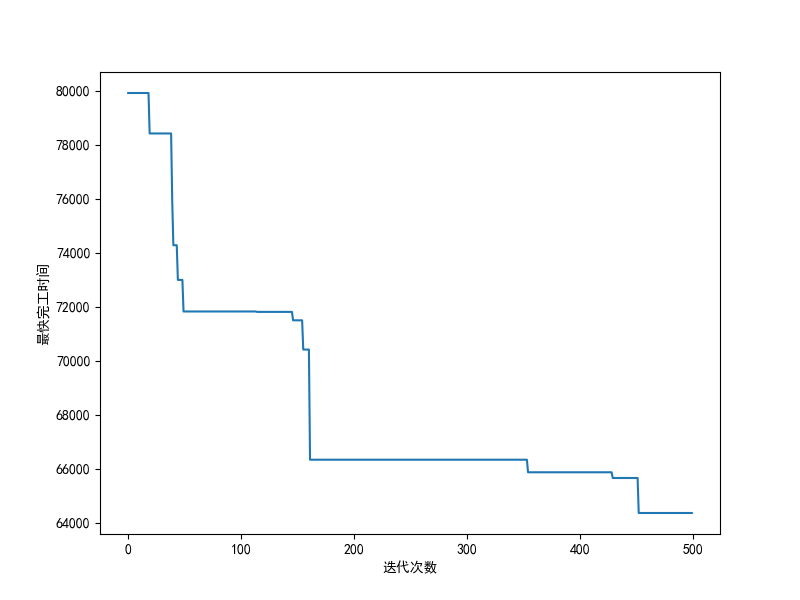
\includegraphics[width=0.8\textwidth]{模型一收敛曲线.png}
		\caption{模型一收敛图}
	\end{figure}

    
    
    
    得到的甘特图如下图所示:

    \begin{figure}[H]
		\centering
		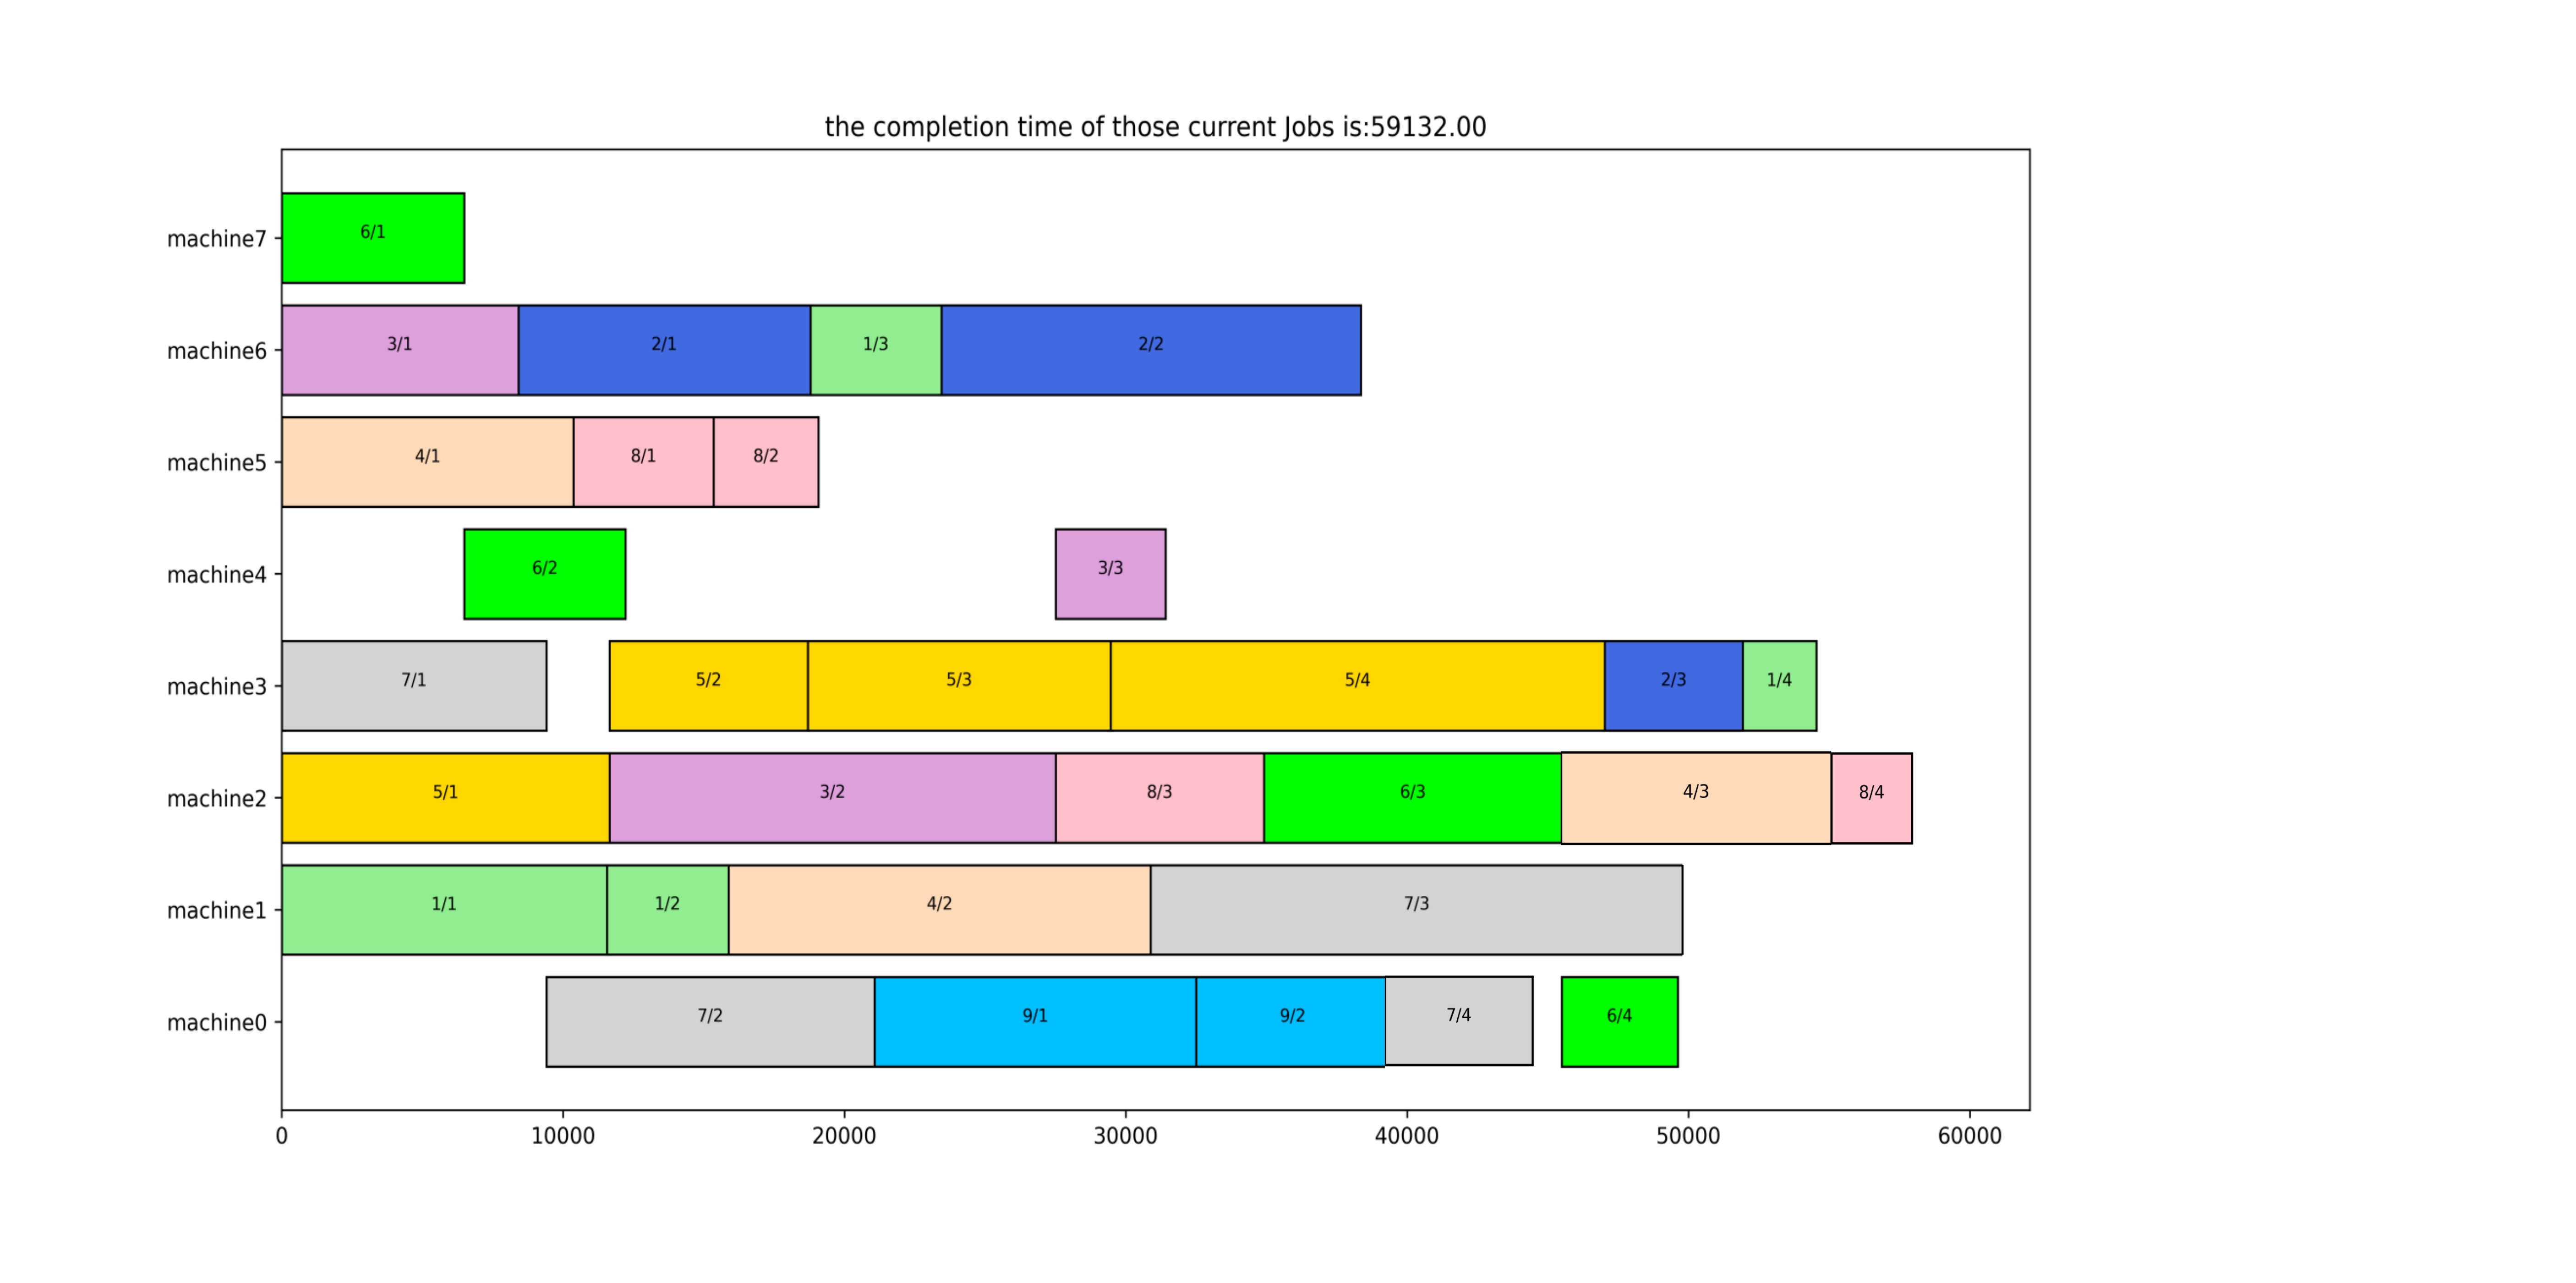
\includegraphics[width=1.2\textwidth]{模型一甘特图.jpg}
		\caption{模型一甘特图}
	\end{figure}

 甘特图是以图示通过活动列表和时间刻度表示出特定项目的顺序,在管理调度统筹中广泛应用。其中纵坐标为机器编号,0-7分别对于A-H,横坐标为加工时间。由图可知,产品加工结束的最优时间为59132分钟,可根据此图进行生产安排规划。

 
    
	\section{问题二模型的建立与求解}
    \subsection{问题二的分析}
    
    基于第一问建立的优化模型,由于可能有产品需要提前交货,所以会增加约束条件,调整目标函数,使得最终满足需要提前交货的产品能够在交货时间之前完成,同时最大完工时间也要尽可能减少。对于提前交货时间不确定的问题,我们利用三角模糊数方法进行分析,再结合第一问的遗传退火算法进行求解。
    
    
    \begin{figure}[H]
        \centering
        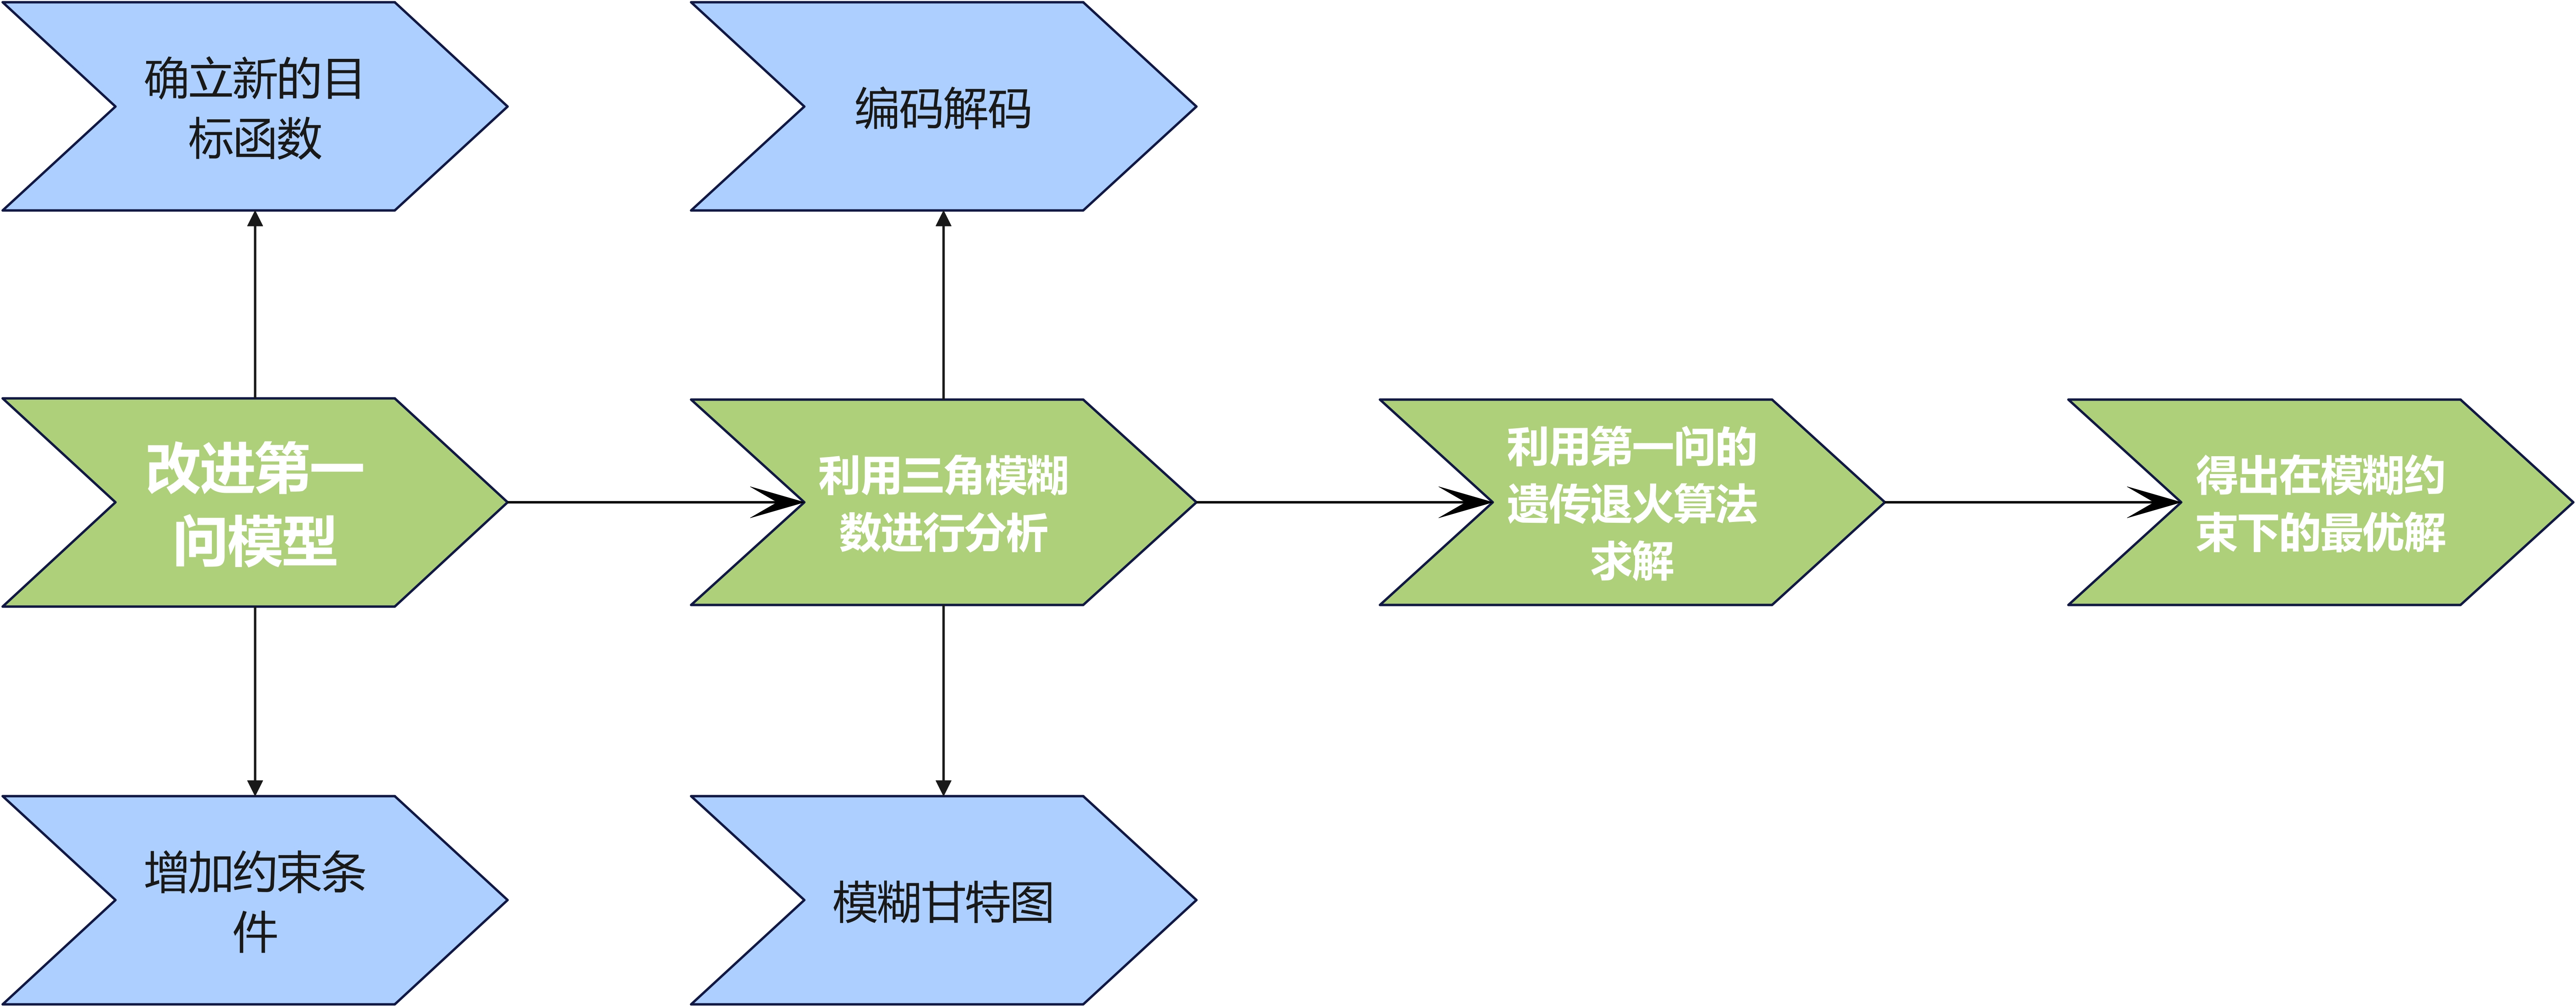
\includegraphics[width=0.9\textwidth]{流程2.jpg}
        \caption{问题二的分析}
    \end{figure}
    
   
    
    \subsection{三角模糊数}
    	
    		\textbf{1.三角模糊数的操作}
      
    		(1)求和:计算每个操作的模糊完成时间。
      
 \begin{gather}
\left.\begin{array}{rl}
\widetilde{A}=\left(a_1, a_2, a_3\right), \widetilde{B} & =\left(b_1, b_2, b_3\right), \widetilde{C}=\left(c_1, c_2, c_3, c_4\right), \widetilde{D}=\left(d_1, d_2, d_3, d_4\right) \\
\widetilde{A}+\widetilde{B} & =\left(a_1+b_1, a_2+b_2, a_3+b_3\right) \\
\widetilde{C}+\widetilde{D} & =\left(c_1+d_1, c_2+d_2, c_3+d_3, c_4+d_4\right)
\end{array}\right\}
\end{gather}

    		(2)取大:计算每个操作的模糊开始时间。

           (3)比较:模糊完成时间是模糊加工时间的总和,因此也变成了三角模糊数,如果要最小化最大的模糊完成时间,就要比较一些模糊完成时间的值。

           准则1:$C_1(\widetilde{A})=\frac{a_{1}+2a_{2}+ a_{3}  }{4} $,根据$C_1$的值 来比较两个模糊数的大小

            准则2: $C_2(\widetilde{A})=a_2$,如果根据$C_1$值无法比较两个模糊数的大小,则根据$C_2$的值来比较大小。

            准则3: $C_3(\widetilde{A})=a_3—a_1$;,如果$C_1$值和$C_2$值都无法比较两个模糊数的大小,则根据$C_3$的值来进行比较\cite{5}。

    	
   	\textbf{2.模糊甘特图} 
   	
   	由于每个操作的开始时间和完成时间都是三角模糊数,因此其甘特图也与正常甘特图不同,如下图,每个操作的模糊开始时间在直线下面,模糊完成时间在直线上面,每个三角形就是前面提到的隶属度函数图像。
   
   
    
    
    
   
    
    \subsection{问题二模型的建立与求解}
     \subsubsection{改进的FJSP模型的建立}
    在这一问题中,考虑到有部分产品需要提前交货,所以建立了新的目标函数如下:
    
    \begin{equation}
    Min\left ( F_{1}  \right ) = \sum_{i=1}^{n} E_{i}   
    \end{equation}
    其中,$E_{i}$为产品i在加工期内加工滞后的程度(单位为分钟),该式表明在满足原有的目标函数和约束条件基础上,要使得各产品在加工期内的滞后时间总和最小,以满足减少最终完工时间的目的。
    
   \begin{equation}
     \sum_{i=1}^{B_{i} } t_{ij} \le 1440T
    \end{equation}

    该式为新增的约束条件,其中$B_{i}$为产品i的交货时间,$t_{ij}$为产品$i$在第$j$天加工的时间,$T$为交货期。该式表示提前要完工的产品需要在交货期之前完成。

   
   对于问题一的双层编码方式,解码时需要通过工序编码和机器编码共同确定具体的调度方案,但这种方法编码序列复杂,且不能保证机器的空闲时间得到充分利用。在求解本问题时,自适应的活动化调度显然更加合适,因此使用基于工序的单层编码:工序编码由$ N $个 $1-n $的工件号组成,每个工件号出现的次数等于其工序数$\mu_{i}$, 执行时按从左到右的顺序安排加工,工件号每出现一次代表该工件遵循工艺流程完成 了一道工序;在机器选择上,使用贪婪策略,选择让当前工序完工时间最小的机器 进行加工,解码时只要工序编码发生变化,机器选择也会随之动态地改变。为了更好理解,给出下表例子进行解释:

   \begin{center}
    	\begin{table}[H]
    		\centering
    		\caption{三角模糊方案实例}
    		\begin{tabular}{ccccc}
    			\toprule[1.5pt]
    			\makebox[0.08\textwidth][c]{工件}	&   
                 \makebox[0.08\textwidth][c]{工序}	&
                 \makebox[0.12\textwidth][c]{$D_1$}	&
    			\makebox[0.12\textwidth][c]{$D_2$}	&
    			\makebox[0.12\textwidth][c]{$D_3$}		\\
    			\midrule[1pt]
    			$J_1$  &   1 &(9353,11553,12553) &	(10553,11625,12325)&	 (11553,12553,13553)  \\
                     & 2 &	(8254,10005,11800) &(4679,5769,6978,) &	(6812,8001,9848)\\
    			    &	3 &	(3958,4657,5657) &(7856,8560,9560) &	(3850,4560,5320) \\
                 $J_2$   &	1 &	(5650,7025,8036) &(8120,9120,10580) &	(9002,11210,12310) \\
                    &	2 &	(13000,14355,16111) &(19830,20018,21032)&	 (17830,19250,21032) \\
                    &	3 &	(9032,9853,10122) &(7053,7895,8950,) &	(9001,9825,11120) \\
                 $J_3$   &	1 &	(5375,6453,7510) &(7123,8150,9120) &	(6150,7223,8130) \\
    			    &	2 &(7860,8390,9125)&(11655,12350,13020)&	(11025,12355,13483)\\
    			
    			\bottomrule[1.5pt]
    		\end{tabular}
    	\end{table}
    \end{center}
   


   假设工序编码为 [1,3,1,3,2,1,2], 编码中第一个“1”代表最先加工工件 1 的第一道工序 $O_{11}$,分配机器时,该工序有 $M_1, M_2,M_3$ 三台机器可以选择,对应的模糊完工时间为 (3,5,8),(7,8,10) 和 (8,9,10),根据模 糊比较准则 (3,5,8) 为最小的完工时间,所以应选择$M_1$ 进行加工;紧跟的“3”代表 $O_{11}$ 之后安排工件 3 的第一道工序 $O_{31}$,该工序也有三台机器可以选择,此时应选择 $M_3$ 加工, 则模糊完工时间为 (2,5,6),要小于选择 $M_1$ 和 $M_2$ 得到的模糊完工时间。之后的工序解码 以此类推,最终可以得到该方案的加工流程:$O_{11}$ → $O_{31}$ → $O_{21}$ → $O_{12}$ → $O_{32}$ →$ O_{13}$ → $O_{22}$, 对应的机器选择为 $N_1$ → $N_3$ →$ N_2$ → $N_1$ →$ N_1$ → $N_3 $→ $N_2$。上述方案用模糊甘特图表示,与时间参数确定的甘特图有所不同,模糊甘特图用下三角和上三角分别表示工序的模糊开始时间和模糊结束时间,若机器在零时刻开始加工首道工序,则零时刻以矩形表示。
   
    

   
    
  
   在加工 $O_{22}$ 时,按照贪婪策略选择了 $N_2$ 为加工机器,尽 管该工序在 $N_1$ 上的模糊加工时间最小,但此之前 $N_1$ 上已经安排了三道工序,如果继 续加大 $N_1$ 的负荷对整个计划的最大完工时间势必有消极影响,且不能有效利用 $N_2$ 的 空闲时间。由此可以看出,对于单目标 FJSP,使用贪婪策略能够更加准确地选出合适 的加工机器,提高设备利用率,同时对比传统的两段编码方式,编码序列也变得更加简单,缓解了算法的优化压力.
    
   
    
   
    
 \subsubsection{利用三角模糊数对FJSP模型的求解}   
     在问题一优化模型中加入了新约束条件后,采用三角模糊算法进行模糊处理,得到的模糊甘特图如图所示。
    
    \begin{figure}[H]
    	\centering
    	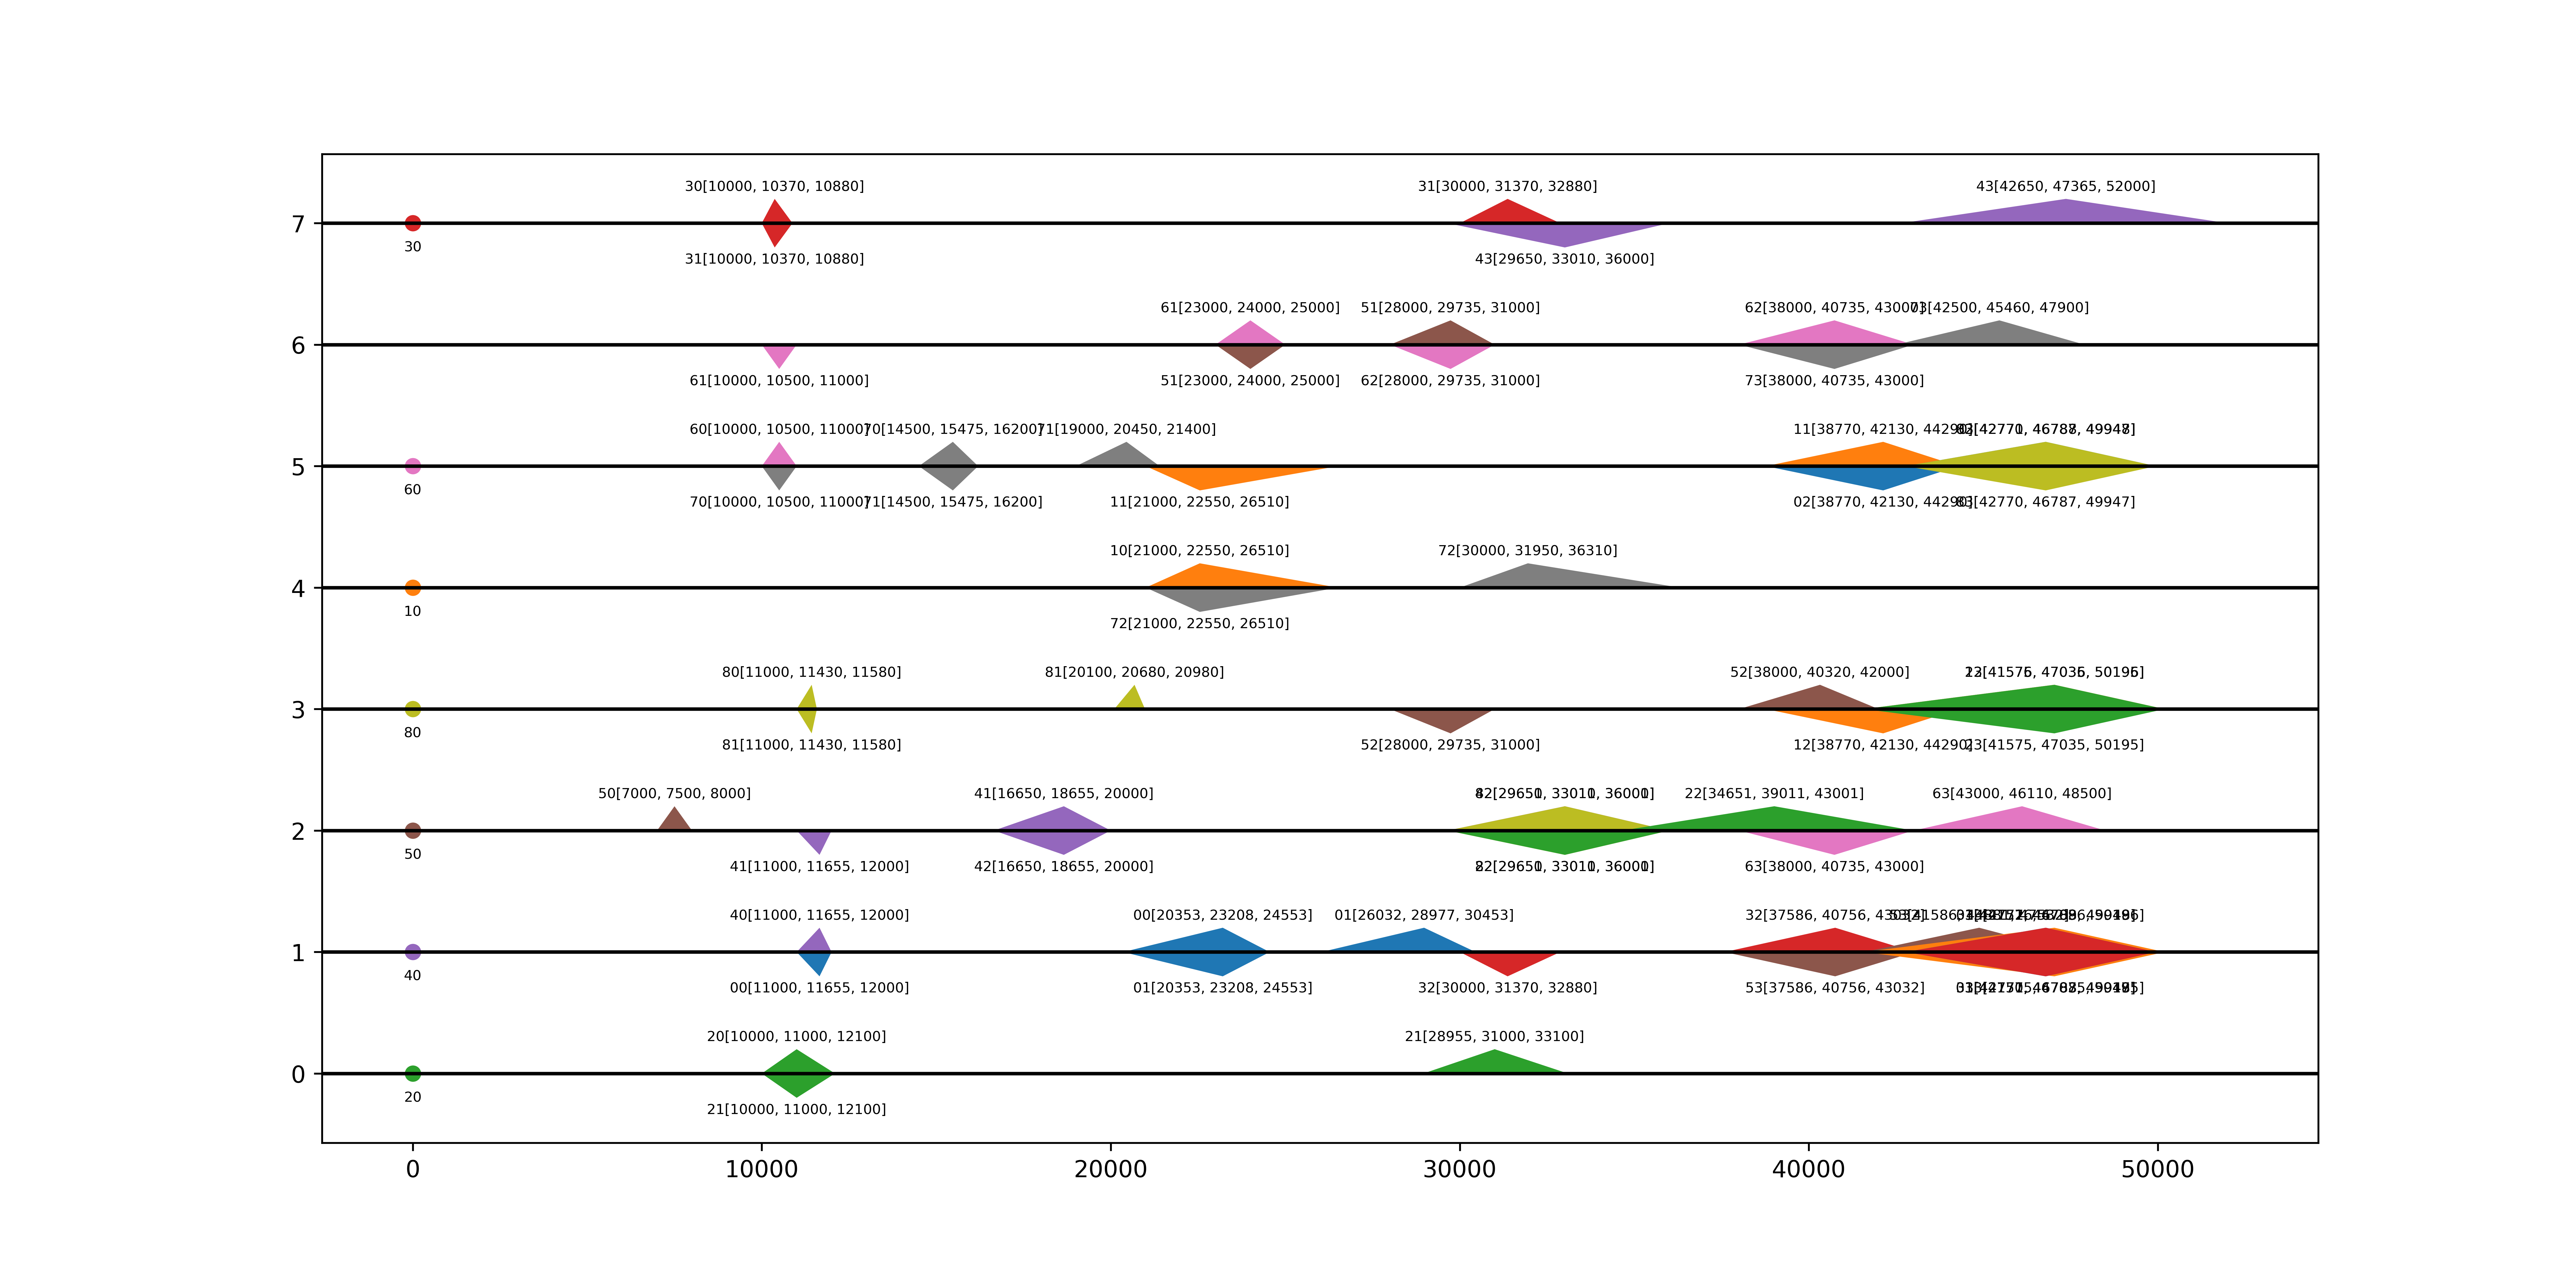
\includegraphics[width=1.0\textwidth]{模糊甘特图.png}
    	\caption{模型二模糊甘特图}
    	
    \end{figure}

    由上图可知,每个小三角形上的数字分别指的是工件的工序数,以及该工件的工序的最早,可能,最晚完成时间。下面用第8个工件的工序加工来进行具体的解释,$o_{70}$[14500,15475,16200]指的是第8个工件的第1道工序在第6台机器上的模糊开始时间为[14500,15475,16200],接下来第8个工件的第2道工序也在第6台机器上进行加工,模糊开始时间为[19000,20450,21400],接下来第8个工件的第3工序在第5台机器上操作有两种可能,而第8个工件的第2道工序和第3道工序不能同时进行,所以第8个工件的第3道工序在第5台机器上加工的模糊开始时间为[30000,31950,36310],最后第8个工件的第4道工序在第7台机器上加工,其模糊开始时间为[38000,40375,43000]。
    
    
    
    \subsection{结果分析}
    由上图可知,每个小三角形上的数字分别指的是工件的工序数,以及该工件的工序的最早,可能,最晚完成时间。下面用第8个工件的工序加工来进行具体的解释,$o_{70}$[14500,15475,16200]指的是第8个工件的第1道工序在第6台机器上的模糊开始时间为[14500,15475,16200],接下来第8个工件的第2道工序也在第6台机器上进行加工,模糊开始时间为[19000,20450,21400],接下来第8个工件的第3工序在第5台机器上操作有两种可能,而第8个工件的第2道工序和第3道工序不能同时进行,所以第8个工件的第3道工序在第5台机器上加工的模糊开始时间为[30000,31950,36310],最后第8个工件的第4道工序在第7台机器上加工,其模糊开始时间为[38000,40375,43000]。
    
     
    
   

    
    \section{问题三模型的建立与求解}
    \subsection{问题三的分析}


问题三要求我们实现高的设备利用率,同时尽快完成产品的加工工作,并在产品数目以及机床数目都可能增加的情况下提出具有一般适用性的生产计划方案。所以该问题为多目标优化类问题,仍考虑问题一的优化模型,改进目标函数并增加约束条件,对问题进行求解并给出合理方案。


    
    
    \subsection{多目标动态规划模型的建立与求解}
   \subsubsection{多目标动态规划模型的建立}
   
     因为该车间既希望减少机器的停工时间,又希望能够实现较短的生产周期,所以便构成了多目标优化\cite{6}的问题。若要满足使各个机床停工时间尽量减少,可对产品进行分批调度,将本月需求的产品分为M批进行生产,可最大化减少机器闲置时间。第三小问在第一小问模型的基础之上进行改进与完善,将使各个机床的停工时间最少这个目标转化为每个工件的最后一道工序在对应的机器上完成的时刻之和最小,改进和完善模型如下:

     首先新增加目标函数:

     \begin{equation}
      min\left ( F_{2}  \right ) = \max_{1\le k\le m}\left \{ \max_{1\le i\le n}\left ( C_{iB_{i}k}- X_{iB_{i}k} \right )   \right \}  
    \end{equation}

    其中$B_i$表示第i个工件的工序数, 

    新增的约束条件:

     \begin{equation}
     H_{ij} =L_{ij} -K_{ij} 
    \end{equation}

    
其中$H_{ij}$指的是第i个工件的第j道工序的切换时间,$K_{ij}$指的是第i个工件的第j道工序开始切换时间,$L_{ij}$指的是第i个工件的第j道工序结束切换时间。这个式子指的是第i个工件的第j道工序的切换时间等于第i个工件的第j道工序结束切换时间与第i个工件的第j道工序开始切换时间之差。

 \begin{equation}
     Z_{i} = \sum_{q=1}^{R_{i} }M_{iq}
    \end{equation}

其中$M_{iq}$指的是第i个产品的第q批次,$R_i$为第i个产品的批次数,该式表明第i个产品本月的需求量为各批次数量之和.

  模型三使机器闲置时间最小化,使机器闲置时间最小化,且产品数目与机器台数可调节,符合一般过程生产情况。

 \subsubsection{多目标动态规化问题的求解}

     基于问题一的遗传退火算法继续解决多目标动态规划问题,新增了目标函数与约束条件进行改进,得到的增加产品数量的甘特图:
     
     \begin{figure}[H]
        \centering
        \includegraphics[width=1\textwidth]{问题三甘特图1.jpg}
        \caption{增加产品数量甘特图}
    \end{figure}

     该图表示了在原先产品数量的基础上数量多了一倍的各机器运作情况,由图可以得出该方案的机器空闲率很低,除了机器三之外,其他机器几乎都一直在运转状态。
     
     
     
     既增加产品数量又增加机器数量的甘特图:

  \begin{figure}[H]
        \centering
        \includegraphics[width=1\textwidth]{问题三甘特图2.jpg}
        \caption{既增加产品数量又增加机器数量甘特图}
    \end{figure}

    对于题目中给出的产量和机器都可能增加的情况,先考虑增加了具体产量的情况,在图中1-1表示工件1的第一批产品,1-2表示工件2的第二批产品.对于考虑既增加产量又增加机器的情况,其中机器编号8表示这台机器是受具体工件产量需求而新增的机器,观察上图可知各个机器空闲率仍然较低,同时得到的最大完工时间的最小值也较低,符合多目标的目标要求。
     
   
  
    
	\section{模型总结与评价}        
        
    
	\subsection{模型总结}
    
    问题一在典型的柔性车间调度问题(FJSP)基础上存在着可以并行加工的工序,需要对传统的FJSP问题的解决方法进行改进。我们需要解决两个问题:确定各作业的加工先后顺序和机器选择。本文利用遗传算法与模拟退火相结合的混合算法,调度优化产品与工序在机器上加工的顺序,使整个系统的加工时间最小。问题二在问题一优化模型的基础上,由于产品需要提前交货,所以会增加约束条件,调整目标函数。对于提前交货时间不确定的问题,我们利用三角模糊数方法进行分析,再结合第一问的遗传退火算法进行求解。问题三为多目标优化类问题,仍考虑问题一的优化模型,新增目标函数和约束条件,对问题进行求解并给出合理方案。
    
	\subsection{模型优缺点分析}
	\subsubsection{模型优点}
	\begin{itemize}
	 \item 将遗传算法与模拟退火算法相结合,取各自算法的优点得到混合算法来求解模型。

  \item 在传统的柔性车间调度问题基础上考虑了可并行的情况,进一步完善了柔性车间调度问题的研究。

    \item 在交叉过程中,相比于以往固定的交叉概率和变异概率,本文采用动态自适应的交叉概率和变异概率,可以加快算法收敛。
    
    \item 问题一建立的遗传退火算法与多个算法进行了对比,是结果最优的算法,证明算法的准确性较高.
	\end{itemize}
   \subsubsection{模型缺点}
	\begin{itemize}
	    \item 并行情况只能考虑该车间的具体情况,并没有较强的通用性。
	    
	    \item 将相同的产品种类进行同一批次的加工来简化模型,不是完全实际的情况.
	\end{itemize}
	\subsection{模型改进}
	  \begin{itemize}
	      \item 寻找更为简单准确的且通用的模型,解决柔性车间调度问题的并行情况.
	      
	     \item 在交叉过程中 ,选取更准确的交叉方式,使得到的结果更有可信度.
	  \end{itemize}
    
	\clearpage

%最后采用的是外面导入bib文件形式
\bibliographystyle{gbt7714-numerical}	%引用样式,参考文献
\bibliography{文献}
\addcontentsline{toc}{section}{参考文献}
%\begin{thebibliography}{}
%\bibitem{}

%\end{thebibliography}
%\addcontentsline{toc}{section}{参考文献}


\clearpage

\appendix %%附录



    
\section{源代码}
\subsection{问题一的求解(python)}
\begin{lstlisting}[language=python]
import numpy as np
import random
from problem import Machine
def encoding(Jobs:list,os:np.array,machines_num:int,stype='GS'):
    '''初始化得到一个解
    机器选择部分有三种初始化方式:全局搜索GS,局部搜索LS,随机搜索RS
    工序排序部分采用随机搜索
    Jobs:工件集
    machines_num:机器总数
    os:初始工序排序部分
    stype:ms初始化方式{GS,LS,RS}
    '''
    ms = np.zeros(len(os),dtype=int) #机器选择编码
    mt = np.zeros(machines_num,dtype=float) #整型数组
    osRecord = 0
    # print('ms:',ms)
    for job in Jobs:
        # 遍历当前工件的工序
        if stype == 'RS':
            for i in range(job.osNum):
                ms[osRecord] = random.randint(0,len(job.minfo[i])-1)
                osRecord += 1
        else:
            for i in range(job.osNum):
                candM = job.minfo[i] #候选机器
                tmpm = mt[candM] + job.tinfo[i] #加工时间相加
                min_val = np.min(tmpm)  # 最小负荷
                min_index = np.argmin(tmpm)  # 获取最小值索引
                mt[candM[min_index]] = min_val
                ms[osRecord] = min_index
                osRecord += 1
            if stype == 'LS':
                mt = np.zeros(machines_num,dtype=float) 
    indexList = list(range(len(os)))
    random.shuffle(indexList)
    return [ms,os[indexList]]



def decoding(s:list,Jobs:list,machines_num=5):
    '''
    s=[ms,os] solution
    ms:机器编码部分
    os:工序排序编码
    Jobs:待加工工件集
    machines_num:机器总数
    returns:
        machines:机器加工信息
        completionT:最后一道工序完工时间
    '''
    ms,os = s[0],s[1]
    machines = [Machine(i) for i in range(machines_num)]
    osCumSum = list(np.cumsum([job.osNum for job in Jobs])) #工件ms分割点
    osCumSum.insert(0,0)

    for num in os:
        # num决定了是第几个工件,job.osCount决定了是工件的第几个工序
        job = Jobs[num]
        if job.osCount == 0:
            jobms = ms[osCumSum[num]:osCumSum[num+1]].copy()
            job.decode(jobms) #解码得到job.Jm和job.T
        
        mId = job.Jm[job.osCount] #工序的机器编号
        mot = job.T[job.osCount]  #工序在该机器上的加工时间
        machines[mId].process(job,mot) #机器加工

 
    completionT = 0
    for machine in machines:
        if machine.processInfo and machine.processInfo[-1].endT > completionT:
            completionT = machine.processInfo[-1].endT

    for job in Jobs:
        job.reset()

    return machines,completionT

    import random
import copy
from problem import Job,visualization
from coding import encoding,decoding
from GA import *
import matplotlib.pyplot as plt

######## 生成算例 ######

machines_num = 10
jobs_num = 18
"""
machine_list = list(range(1,machines_num+1))
products = ['A','B','C','D','E','F']    #设置每一种产品对应一种颜色
colors = ['r','g','b','c','m','y','k','w']
ptocolor = dict(zip(products, colors))
Jobs = []
Joblists = []
Ts = []
for i in range(jobs_num): # 遍历每一个工件
    onum = 4 # 工序数
    candMs = [] # 可选机器数字
    candTs = [] # 所化时间
    for j in range(onum):
        mnum = random.randint(1,machines_num) #工序可选机器数
        candm = random.sample(machine_list,mnum)
        candMs.append(candm) # 添加某一道工序可选择的机器
        #工序在不同机器上对应的加工时间
        candt = [random.randint(1,10) for _ in candm] #某道工艺在某台机器上的时间
        candTs.append(candt) # 添加某一道工序在不同机器上的加工时间
    Joblists.append(candMs) # 可选机器数字
    Ts.append(candTs)
    productType = products[random.randint(0,len(products)-1)]
    Jobs.append(Job(i+1,candMs,candTs,productType))
"""
products = ['A','B','C','D','E','F','G','H','I']    #设置每一种产品对应一种颜色
colors = ['lightgreen','royalblue','plum','peachpuff','gold','lime','lightgrey','pink','deepskyblue']
ptocolor = dict(zip(products, colors))
Job1 = Job('1-1', minfo=[[2,3,4,10], [2,3,4,9,10], [6,7,9,10], [2,3,4,9,10]], tinfo=[[11553,11553,11553,11553], [5769,5769,5769,5769,5769], [4657,4657,4657,4657], [2616,2616,2616,2616,2616]], productType='A')
Job2 = Job('2-1', minfo=[[6,7,9,10], [6,7,9,10], [2,3,4,9,10]], tinfo=[[10380,10380,10380,10380], [14910,14910,14910,14910], [4905,4905,4905,4905,4905]], productType='B')
Job3 = Job('3-1', minfo=[[5,6,7,8,9,10], [2,3,4,9,10], [5,6,7,8,9,10]], tinfo=[[8410,8410,8410,8410,8410,8410], [15855,15855,15855,15855,15855], [3902,3902,3902,3902,3902,3902]], productType='C')
Job4 = Job('4-1', minfo=[[5,6,7,9,10], [2,3,4,9,10], [2,3,4,9,10]], tinfo=[[10370,10370,10370,10370,10370], [15000,15000,15000,15000,15000], [9386,9386,9386,9386,9386]], productType='D')
Job5 = Job('5-1', minfo=[[1,2,3,4,9,10], [1,2,3,4,9,10], [1,2,3,4,9,10], [2,3,4,9,10]], tinfo=[[11655,11655,11655,11655,11655,11655], [7043,7043,7043,7043,7043,7043], [14355,14355,14355,14355,14355,14355], [23410,23410,23410,23410,23410]], productType='E')
Job6 = Job('6-1', minfo=[[5,6,7,8,9,10], [5,6,7,8,9,10], [2,3,9,10], [1,2,3,4,9,10]], tinfo=[[6480,6480,6480,6480,6480,6480], [5735,5735,5735,5735,5735,5735], [10585,10585,10585,10585], [4125,4125,4125,4125,4125,4125]], productType='F')
Job7 = Job('7-1', minfo=[[1,2,3,4,9,10], [1,2,3,4,9,10], [2,3,4,9,10], [1,2,3,4,9,10]], tinfo=[[9405,9405,9405,9405,9405,9405], [11665,11665,11665,11665,11665,11655], [18910,18910,18910,18910,18910], [5375,5375,5375,5375,5355,5355]], productType='G')
Job8 = Job('8-1', minfo=[[5,6,7,8,9,10], [5,6,7,8,9,10], [2,3,4,9,10], [1,2,3,4,9,10]], tinfo=[[4975,4975,4975,4975,4975,4975], [4975,4975,4975,4975,4975,4975], [7395,7395,7395,7395,7396], [2875,2875,2875,2875,2875,2875]], productType='H')
Job9 = Job('9-1', minfo=[[1,2,3,4,9,10], [1,2,3,4,9,10]], tinfo=[[11430,11430,11430,11430,11430,11430], [9155,9155,9155,9155,9155,9155]], productType='I')
Job11 = Job('1-2', minfo=[[2,3,4], [2,3,4], [6,7], [2,3,4]], tinfo=[[11553,11553,11553], [5769,5769,5769], [4657,4657], [2616,2616,2616]], productType='A')
Job22 = Job('2-2', minfo=[[6,7,], [6,7], [2,3,4]], tinfo=[[10380,10380], [14910,14910], [4905,4905,4905]], productType='B')
Job33 = Job('3-2', minfo=[[5,6,7,8], [2,3,4], [5,6,7,8]], tinfo=[[8410,8410,8410,8410], [15855,15855,15855], [3902,3902,3902,3902]], productType='C')
Job44 = Job('4-2', minfo=[[5,6,7,9], [2,3,4], [2,3,4]], tinfo=[[10370,10370,10370,10370], [15000,15000,15000], [9386,9386,9386]], productType='D')
Job55 = Job('5-2', minfo=[[1,2,3,4], [1,2,3,4], [1,2,3,4], [2,3,4]], tinfo=[[11655,11655,11655,11655], [7043,7043,7043,7043], [14355,14355,14355,14355], [23410,23410,23410]], productType='E')
Job66 = Job('6-2', minfo=[[5,6,7,8], [5,6,7,8], [2,3,4], [1,2,3,4]], tinfo=[[6480,6480,6480,6480], [5735,5735,5735,5735], [10585,10585,10585], [4125,4125,4125,4125]], productType='F')
Job77 = Job('7-2', minfo=[[1,2,3,4], [1,2,3,4], [2,3,4], [1,2,3,4]], tinfo=[[9405,9405,9405,9405], [11665,11665,11665,11665], [18910,18910,18910], [5375,5375,5375,5375]], productType='G')
Job88 = Job('8-2', minfo=[[5,6,7,8], [5,6,7,8], [2,3,4], [1,2,3,4]], tinfo=[[4975,4975,4975,4975], [4975,4975,4975,4975], [7395,7395,7395], [2875,2875,2875,2875]], productType='H')
Job99 = Job('9-2', minfo=[[1,2,3,4], [1,2,3,4]], tinfo=[[11430,11430,11430,11430], [9155,9155,9155,9155]], productType='I')
Jobs = [Job1,Job2,Job3,Job4,Job5,Job6,Job7,Job8,Job11,Job22,Job33,Job44,Job55,Job66,Job77,Job88,Job99]
Joblists = [[[2,3,4], [2,3,4], [6,7], [2,3,4]], [[6,7], [6,7], [2,3,4], [1]], [[5,6,7,8], [2,3,4], [5,6,7,8], [1]], [[5,6,7], [2,3,4], [2,3,4], [1]], [[1,2,3,4], [1,2,3,4], [1,2,3,4], [2,3,4]], [[5,6,7,8], [5,6,7,8], [2,3,4], [1,2,3,4]], [[1,2,3,4], [1,2,3,4], [2,3,4], [1,2,3,4]], [[5,6,7,8], [5,6,7,8], [2,3,4], [1,2,3,4]], [[1,2,3,4], [1,2,3,4], [1], [1]]]
Ts = [[[11553,11553,11553], [5769,5769,5769], [4657,4657], [2616,2616,2616]], [[17380,17380], [19770,19770], [4905,4905,4905], [1]], [[8410,8410,8410,8410], [15855,15855,15855], [3902,3902,3902,3902], [1]], [[10370,10370,10370], [10000,10000,10000], [9386,9386,9386], [1]], [[11655,11655,11655,11655], [7043,7043,7043,7043], [14355,14355,14355], [23410,23410,23410]], [[6480,6480,6480,6480], [5735,5735,5735,5735], [10585,10585,10585], [4125,4125,4125,4125]], [[9405,9405,9405,9405], [11665,11665,11665], [18910,18910,18910], [5375,5375,5375]], [[4975,4975,4975,4975], [4975,4975,4975,4975], [7395,7395,7395], [2875,2875,2875]], [[11430,11430,11430,11430], [9155,9155,9155,9155], [1], [1]]]

jobSequence = list(range(jobs_num))
allOT = []
for job in Jobs:
    allOT.extend(job.tinfo)
os = []
for i,job in enumerate(Jobs):
    for j in range(job.osNum):
        os.append(i)
os = np.array(os)
rs = list(range(len(os))) #位点列表





######## 算法求解 #######

# 遗传算法参数
popSize = 50 #总群大小
maxGen = 500 #迭代次数
pc = 0.75  #交叉概率
pm = 0.2  #变异概率


# 生成初始种群


population = initializePopulation(Jobs,os,machines_num,popSize)
for individual in population:
    if individual.fit is None:
        _,individual.fit = decoding(individual.s,Jobs,machines_num)
bestS = copy.deepcopy(getbest(population))
bestfits = [bestS.fit]
gen = 0
while gen < maxGen:
    fitness = [ 1 / individual.fit for individual in population]
    cumSum = np.cumsum(fitness)
    fitnessratio = cumSum / cumSum[-1]
    parents = [] 
    for i in range(popSize):
        parents.append(selection(population,fitnessratio))
    population = parents.copy()
    # 交叉
    for i in range(popSize):
        if random.random() < pc:
            P1 = population[i].s
            j = random.randint(0,popSize-1)
            P2 = population[j].s
            C1,C2 = cross(P1,P2,rs,jobSequence)
            population[i].s,population[i].fit = C1,None
            population[j].s,population[j].fit = C2,None

    # 变异
    for i in range(popSize):
        if random.random() < pm:
            population[i].s = mutation(population[i].s,rs,allOT)
            population[i].fit = None
    
        if population[i].fit is None:
            _,population[i].fit = decoding(population[i].s,Jobs,machines_num)
    
    curbestS = getbest(population)
    if curbestS.fit <= bestS.fit:
        bestS = copy.deepcopy(curbestS)
    else:
        population[0] = copy.deepcopy(bestS)
    bestfits.append(bestS.fit)
    gen += 1

machines,completionT = decoding(bestS.s,Jobs,machines_num)
plt.plot(bestfits)
plt.show()
# for machine in machines:
#     for info in machine.processInfo:
#         print(info)
# 可视化车间调度结果
visualization(machines,completionT,ptocolor,machines_num)


import numpy as np
import random
from coding import encoding,decoding


class Solution:
    def __init__(self,s) -> None:
        self.s = s
        self.fit = None


###### 遗传算法求解FJSP算子设计 ######

#1.种群初始化
def initializePopulation(Jobs,os,machines_num=8,popSize=100):
    '''初始化总群'''
    population = [Solution(encoding(Jobs,os,machines_num,stype='GS')),
                  Solution(encoding(Jobs,os,machines_num,stype='LS'))
                  ]    
    for i in range(2,popSize):
        population.append(Solution(encoding(Jobs,os,machines_num,stype='RS')))
    
    return population

#2.选择
def selection(population:list,fitnessratio):
    '''轮盘赌选择
    population:种群[individual]
    fitness:种群个体对应的适应度
    return:
        best:当前锦标赛中最好的个体
    '''
    r = random.random()
    target_idx = np.where(fitnessratio >= r)[0][0]
    return population[target_idx]

def getbest(population):
    '''找出当前种群中最好的个体及其适应度
    '''
    fitness = [individual.fit for individual in population]
    bestidx = np.argmin(fitness)
    bestS = population[bestidx]
    return bestS

#3.交叉
def cross(P1:list,P2:list,rs:list,jobSequence:list):
    '''
    P1,P2 [ms,os]
    rs:机器选择位点rs=list(range(工序总数))
    jobSequence:工件当前在Jobs列表中的的相对顺序=list(range(工件总数))
    '''
    def mscross(ms1:np.array,ms2:np.array,rs:list):
        '''均匀交叉
        ms1,ms2:父代机器选择部分
        rs:机器选择位点rs=list(range(工序总数))
        '''
        r = random.randint(1,len(rs))
        # crossIndex = sorted(random.sample(rs,r)) #交叉位点
        crossIndex = random.sample(rs,r) #交叉位点
        c1,c2 = ms1.copy(),ms2.copy()
        c1[crossIndex],c2[crossIndex] = c2[crossIndex],c1[crossIndex]
        
        return c1,c2
    def oscross(os1:np.array,os2:np.array,jobSequence:list):
        '''POX交叉'''
        def generate_offspring(os1,os2,c):
            i,j = 0,0
            while i < len(os2):
                if os2[i] not in crossIds:
                    while j < len(os1):
                        if os1[j] not in crossIds:
                            c[j] = os2[i]
                            j += 1
                            break
                        j += 1
                i += 1
            return c
        r = random.randint(1,len(jobSequence)) #将工作集合一分为2
        crossIds = sorted(random.sample(jobSequence,r)) #交叉元素
        c1,c2 = os1.copy(),os2.copy()
        c1 = generate_offspring(os1,os2,c1)
        c2 = generate_offspring(os2,os1,c2)
        
        return c1,c2
    
    msc1,msc2 = mscross(P1[0],P2[0],rs)
    osc1,osc2 = oscross(P1[1],P2[1],jobSequence)
    C1,C2 = [msc1,osc1],[msc2,osc2]
    return C1,C2

#4.变异
def mutation(s,rs,allOT):
    def msmutation(ms,rs,allOT):
        '''
        Step1:在变异染色体中随机选择r个位置
        Step2:依次选择每一个位置,对每一个位置的机器设置为当前工序可选机器集合加工时间最短的机器
        ms:机器选择部分编码
        rs:list(range(工序总数))
        allOT:当前排序下所有工序的时间矩阵
        '''
        r = random.randint(1,len(rs))
        mutaionIndex = random.sample(rs,r) #变异位点        
        for i in mutaionIndex:
            ms[i] = np.argmin(allOT[i])
        
        return ms
        
    def osmutation(os):
        '''
        随机选择两个位点进行转置
        '''
        osIndex = list(range(len(os)))
        a,b = sorted(random.sample(osIndex,2))
        if b == len(osIndex):
            b += 1
        temp = list(os[a:b])
        temp.reverse()
        os[a:b] = temp
        return os
    s[0] = msmutation(s[0],rs,allOT)
    s[1] = osmutation(s[1])
    return s


import numpy as np
import matplotlib.pyplot as plt

class Job:
    def __init__(self,jobId:str,minfo:list,tinfo:list,productType:str) -> None:
        self.id = jobId    #工件名字
        self.osNum = len(minfo) #工件的工序数
        self.minfo = self.list_to_array(minfo) #工件每个工序可选择的加工机器
        self.tinfo = self.list_to_array(tinfo,infotype='t') #工件每个工序在不同机器上的加工时间
        self.productType = productType #工件所属产品型号
        self.osCount = 0 #加工工序次序
        self.startTs = [0] #工序开始加工时间
        self.endTs = [0]   #工序加工结束时间
    


    def list_to_array(self,listinfo:list,infotype='m'):
        info = listinfo.copy()
        if infotype == 'm':
            for i in range(self.osNum):
                info[i] = np.array(info[i]) - 1 #python的索引从0开始
        else:
            for i in range(self.osNum):
                info[i] = np.array(info[i])
        return info
    
    def decode(self,ms:np.array):
        '''解码机器顺序矩阵和时间矩阵顺序'''
        Jm,T = [],[]
        for i in range(self.osNum):
            Jm.append(self.minfo[i][ms[i]])
            T.append(self.tinfo[i][ms[i]])
        self.Jm,self.T = Jm,T
        return Jm,T
    
    def updateT(self,startT,endT):
        '''更新工件工序的加工开始时间和加工结束时间
        startT:工序加工开始时间
        operationT:工序加工结束时间
        '''
        self.startTs.append(startT)
        self.endTs.append(endT)
        self.osCount += 1


    def reset(self):
        '''重置时间'''
        self.startTs = [0]
        self.endTs = [0]
        self.osCount = 0

class WorkInfo:
    def __init__(self,startT=None,duration=None,endT=None,jobid=None,joboreder=None,jobtype=None):
        self.startT = startT            #状态开始时间
        self.duration = duration        #状态持续时间
        self.endT = endT                #状态结束时间
        self.jobid = jobid              #工件编号
        self.joborder = joboreder       #工件次序
        self.jobtype = jobtype          #工件类属产品
    
    def __str__(self):
        return f"开始加工时间:{self.startT},加工持续时间:{self.duration},加工结束时间:{self.endT},工件编号:{self.jobid},工件次序:{self.joborder},工件类属产品:{self.jobtype}"
class Machine:
    def __init__(self,id):
        self.id = id #机器编号
        self.processInfo = [] #[开始加工时间,加工时间,加工结束时间,工件编号,工件工序号,工件产品类型]

    def process(self,job,mot):
        '''工件工序的加工操作
        jobid:工件编号
        mot:机器加工该工件当前工序的耗时
        '''
        if self.processInfo:
            startT = max(job.endTs[-1],self.processInfo[-1].endT)
            if startT == self.processInfo[-1].endT and \
                job.productType == self.processInfo[-1].jobtype:#连续
                mot *= 0.75
        else:
            startT = job.endTs[-1]
        endT = startT + mot
        job.updateT(startT,endT)    
        workinfo = WorkInfo(startT,mot,endT,jobid=job.id,joboreder=job.osCount,jobtype=job.productType)
        self.processInfo.append(workinfo)
    
    def reset(self):
        '''重置'''
        self.processInfo = []

# 绘制甘特图
def visualization(machines,completionT,ptocolor,machines_num=5):
    '''绘制甘特图
    '''
    plt.figure(figsize=(len(machines)*5,len(machines)))
    # 设置清晰度
    plt.rcParams['savefig.dpi'] = 500
    for i in range(machines_num):
        for osProcessInfo in machines[i].processInfo:
            plt.barh(i, width=osProcessInfo.duration, height=0.8, left=osProcessInfo.startT,align='center',
                         color=ptocolor[osProcessInfo.jobtype], edgecolor='k')
            plt.text(x=osProcessInfo.startT + osProcessInfo.duration/2, y=i, s=f"{osProcessInfo.jobid}/{osProcessInfo.joborder}",
                         horizontalalignment='center',fontsize=8)
    plt.yticks(list(range(machines_num)),
           ['machine%d'%i for i in range(machines_num)])
    plt.title('the completion time of those current Jobs is:%.2f'%59132)
    plt.show()



    
\end{lstlisting}













\subsection{问题二、问题三模型求解(python)}
\begin{lstlisting}[language=python]
import numpy as np
import random
from params import get_args
from Shop import Shop
from utils import *


class GA(object):
    def __init__(self, args, shop):
        self.shop = shop
        self.cross_rate = args.cross_rate
        self.mutate_rate = args.mutate_rate
        self.pop_size = args.pop_size
        self.elite_number = args.elite_number

        self.chrom_size = self.shop.job_nb * self.shop.op_nb
        self.pop = []

    def encode(self):
        init_pop = []
        for _ in range(self.pop_size):
            one_string = []
            for _ in range(self.shop.op_nb):
                one_string += list(np.random.permutation(self.shop.job_nb))
            random.shuffle(one_string)
            two_string = [random.randint(0, self.shop.machine_nb-1) for _ in range(self.chrom_size)]
            individual = np.vstack([one_string, two_string])
            init_pop.append(individual)
        return np.array(init_pop)

    def decode(self, pop1):
        fuzzy_fitness = []
        certain_fitness = []
        for individual in pop1:
            fuzzy_completion_time = self.shop.process_decode1(individual)
            fuzzy_fitness.append(fuzzy_completion_time)
            certain_fitness.append(value(fuzzy_completion_time))
        return fuzzy_fitness, certain_fitness

    def selection(self, pop2, fuzzy_fitness, certain_fitness):
        """
        tournament selection + elite_strategy
        """
        pop2 = pop2.tolist()
        sorted_pop = sorted(pop2, key=lambda x: certain_fitness[pop2.index(x)], reverse=False)
        new_pop = sorted_pop[:self.elite_number]
        while len(new_pop) < self.pop_size:
            index1, index2 = random.sample(list(range(10, self.pop_size)), 2)
            if rank(fuzzy_fitness[index1], fuzzy_fitness[index2]) == fuzzy_fitness[index1]:
                new_pop.append(pop2[index2])
            else:
                new_pop.append(pop2[index1])
        return np.array(new_pop)

    def crossover_machine(self, pop_machine):
        """
        two point crossover (TPX)
        """
        temp = pop_machine.copy().tolist()
        new_pop = []
        while len(temp) != 0:
            parent1, parent2 = random.sample(temp, 2)
            temp.remove(parent1)
            temp.remove(parent2)
            if random.random() < self.cross_rate:
                pos1, pos2 = sorted(random.sample(list(range(self.chrom_size)), 2))
                offspring1 = parent1[:pos1] + parent2[pos1:pos2] + parent1[pos2:]
                offspring2 = parent2[:pos1] + parent1[pos1:pos2] + parent2[pos2:]
            else:
                offspring1 = parent1
                offspring2 = parent2
            new_pop.append(offspring1)
            new_pop.append(offspring2)
        return np.array(new_pop)

    def crossover_job(self, pop_job):
        """
        generalisation of the precedence preservative crossover (PPX)
        """
        temp = pop_job.copy().tolist()
        new_pop = []
        for parent1 in temp:
            if random.random() < self.cross_rate:
                new_individual = []
                parent2 = pop_job[random.randint(0, self.pop_size-1)].tolist()
                string = random.choices([0, 1], k=self.chrom_size)
                for choose in string:
                    if int(choose) == 0:
                        new_individual.append(parent1[0])
                        parent2.remove(parent1[0])
                        parent1 = parent1[1:]
                    else:
                        new_individual.append(parent2[0])
                        parent1.remove(parent2[0])
                        parent2 = parent2[1:]
                new_pop.append(new_individual)
            else:
                new_pop.append(parent1)
        return np.array(new_pop)

    def mutation(self, part):
        """
        swap
        """
        for individual in part:
            if random.random() < self.mutate_rate:
                pos1, pos2 = random.sample(list(range(self.chrom_size)), 2)
                individual[pos1], individual[pos2] = individual[pos2], individual[pos1]
        return part

    @staticmethod
    def elite_strategy(pop3, fitness):
        best_fitness = [np.inf, np.inf, np.inf]
        best_individual = None
        for k, individual in enumerate(pop3):
            if rank(fitness[k], best_fitness) == best_fitness:
                best_fitness = fitness[k]
                best_individual = individual
        return best_individual, best_fitness


if __name__ == '__main__':
    args = get_args()
    job, machine, op, pt = read('./instance2.txt')
    shop = Shop(job, machine, op, pt)
    method = GA(args, shop)

    best_one = None
    best_fit = [np.inf, np.inf, np.inf]

    best_list = []
    mean_list = []

    pop = method.encode()
    for i in range(args.max_generation):
        fuzzy_fit, certain_fit = method.decode(pop)
        new_one, new_fit = method.elite_strategy(pop, fuzzy_fit)
        if i % 100 == 0:
            print(f'{i}:old best:{best_fit}, now best:{new_fit}, now mean:{np.mean(certain_fit)}')
        if rank(best_fit, new_fit) == best_fit:
            best_fit = new_fit
            best_one = new_one
        best_list.append(value(best_fit))
        mean_list.append(np.mean(certain_fit))

        pop_select = method.selection(pop, fuzzy_fit, certain_fit)
        pop_cross_job = method.crossover_job(pop_select[:, 0, :])
        pop_mutate_job = method.mutation(pop_cross_job)
        pop_cross_machine = method.crossover_machine(pop_select[:, 1, :])
        pop_mutate_machine = method.mutation(pop_cross_machine)
        new = []
        for a, b in zip(pop_mutate_job, pop_mutate_machine):
            new.append([a, b])
        pop = np.array(new)
    fct = shop.process_decode1(best_one)
    shop.draw_fuzzy_gantt()
    draw(best_list, mean_list)



from utils import *
import matplotlib.pyplot as plt
import matplotlib.colors as mc


class Job(object):
    def __init__(self, index, op_nb, total_fuzzy_pt):
        self.index = index
        self.op_nb = op_nb
        self.fuzzy_pt = total_fuzzy_pt[index]

        self.current_op = 0
        self.current_time = [0, 0, 0]

    def process(self, start_time, process_time):
        self.current_op += 1
        self.current_time = addition(start_time, process_time)


class Machine(object):
    def __init__(self, index):
        self.index = index
        self.current_time = [0, 0, 0]

        self.op_start_time = []
        self.op_end_time = []
        self.job_index = []
        self.op_index = []

    def process(self, start_time, process_time, job_index, op_index):
        self.current_time = addition(start_time, process_time)
        self.op_start_time.append(start_time)
        self.op_end_time.append(self.current_time)
        self.job_index.append(job_index)
        self.op_index.append(op_index)


class Shop(object):
    def __init__(self, job_nb, machine_nb, op_nb, total_fuzzy_pt):
        self.job_nb = job_nb
        self.machine_nb = machine_nb
        self.op_nb = op_nb
        self.total_fuzzy_pt = total_fuzzy_pt

        self.job_list = []
        self.machine_list = []

    def create(self):
        self.job_list = []
        self.machine_list = []
        for i in range(self.job_nb):
            self.job_list.append(Job(i, self.op_nb, self.total_fuzzy_pt))
        for i in range(self.machine_nb):
            self.machine_list.append(Machine(i))

    def process_decode1(self, solution):
        self.create()
        op_se, ma_se = solution[0], solution[1]
        for k in range(len(op_se)):
            job_index = op_se[k]
            job = self.job_list[job_index]
            machine_index = ma_se[k]
            machine = self.machine_list[machine_index]
            start_time = rank(job.current_time, machine.current_time)
            process_time = job.fuzzy_pt[job.current_op][machine_index]
            machine.process(start_time, process_time, job_index, job.current_op)
            job.process(start_time, process_time)
        fuzzy_completion_time = [0, 0, 0]
        for ma in self.machine_list:
            fuzzy_completion_time = rank(fuzzy_completion_time, ma.current_time)
        return fuzzy_completion_time

    def draw_fuzzy_gantt(self):
        plt.figure(figsize=(12, 8))
        # 调整清晰度
        plt.rcParams['savefig.dpi'] = 600
        colors = list(mc.TABLEAU_COLORS.keys())
        for ma in self.machine_list:
            y = ma.index
            plt.axhline(y, color='black')
            plt.yticks(list(range(self.machine_nb)))
            for k, start, end, o in zip(ma.job_index, ma.op_start_time, ma.op_end_time, ma.op_index):
                if start == [0, 0, 0]:
                    plt.scatter(0, y, color=colors[k])
                    plt.text(start[1], y-0.2, str(k)+str(o), verticalalignment='center', horizontalalignment='center',
                             fontsize=6)
                else:
                    triangleX = start
                    triangleY = [y, y-0.2, y]
                    plt.fill(triangleX, triangleY, colors[k])
                    plt.text(start[1], y-0.3, str(k)+str(o)+str(start), verticalalignment='center', horizontalalignment='center',
                             fontsize=6)
                triangleX = end
                triangleY = [y, y+0.2, y]
                plt.fill(triangleX, triangleY, colors[k])
                plt.text(end[1], y+0.3, str(k)+str(o)+str(end), verticalalignment='center', horizontalalignment='center', fontsize=6)
        plt.show()


import numpy as np
import matplotlib.pyplot as plt

"""
(1) fuzzy operators
"""


def addition(s1, s2):
    a = s1[0] + s2[0]
    b = s1[1] + s2[1]
    c = s1[2] + s2[2]
    return [a, b, c]


def old_max(s1, s2):
    a = max(s1[0], s2[0])
    b = max(s1[1], s2[1])
    c = max(s1[2], s2[2])
    return [a, b, c]


def value(s):
    return (s[0] + 2 * s[1] + s[2]) / 4


def rank(s1, s2):
    if value(s1) > value(s2):
        return s1
    elif value(s1) < value(s2):
        return s2
    elif s1[1] > s2[1]:
        return s1
    elif s1[1] < s2[1]:
        return s2
    elif (s1[2] - s1[0]) > (s2[2] - s2[0]):
        return s1
    else:
        return s2


"""
(2) read instance
"""


def read(path):
    with open(path) as file:
        lines = file.read().split('\n')
    part = lines[0].split()
    job_nb, machine_nb, op_nb = int(part[0]), int(part[1]), int(part[2])

    job_fuzzy_pt = []
    total_fuzzy_pt = []

    for k in range(1, job_nb * op_nb + 1):
        line = lines[k]
        part = line.split()
        pt = [list(map(int, x)) for x in [a.split(',') for a in part[1:]]]
        job_fuzzy_pt.append(pt)
        if len(job_fuzzy_pt) == op_nb:
            total_fuzzy_pt.append(job_fuzzy_pt)
            job_fuzzy_pt = []
    return job_nb, machine_nb, op_nb, np.array(total_fuzzy_pt)


"""
(3) valid
"""


def check_valid(pop, op_nb, job_nb):
    pop = pop.tolist()
    for p in pop:
        for i in range(job_nb):
            if p.count(i) != op_nb:
                print('error')
    print('right')


"""
(4) plot
"""


def draw(best, mean):
    plt.figure()
    plt.plot(best, label='best')
    plt.plot(mean, label='mean')
    plt.xlabel('generation')
    plt.ylabel('fitness')
    plt.legend()
    plt.show()


import argparse


def get_args():
    parser = argparse.ArgumentParser(description="hyper parameters")

    parser.add_argument('--cross_rate', default=0.8, type=int, help='cross_rate')
    parser.add_argument('--mutate_rate', default=0.1, type=int, help='mutate_rate')
    parser.add_argument('--pop_size', default=100, type=int, help='pop_size')
    parser.add_argument('--max_generation', default=1000, type=int, help='max_generation')
    parser.add_argument('--elite_number', default=10, type=int, help='elite_strategy')

    args = parser.parse_args()
    return args

\end{lstlisting}



 
\end{spacing}
\end{document}